\documentclass{book}

\usepackage[a5paper,margin=0.70cm,includeheadfoot]{geometry}
% \geometry{showframe}

\usepackage[hyphens,allowmove]{url}
\usepackage[colorlinks=true,linkcolor=blue,urlcolor=blue,citecolor=black,breaklinks,pdftex]{hyperref}
\urlstyle{same}
\makeatletter
  \begingroup
    \endlinechar=-1 %
    \catcode`\^^A=14 %
    \catcode`\^^M\active
    \catcode`\%\active
    \catcode`\#\active
    \catcode`\_\active
    \catcode`\$\active
    \catcode`\&\active
    \let\my@url\hyper@normalise
    \patchcmd\my@url{\hyper@n@rmalise}{\my@url@}{}{}^^A
    \global\let\my@url\my@url
  \endgroup
  \DeclareRobustCommand*\my@url@[2][]{\endgroup\href{#1#2}{\nolinkurl{#2}}}
  \DeclareRobustCommand*\url{\my@url}
  \g@addto@macro{\UrlBreaks}{\do\/\do\-} 
\makeatother
\usepackage[hyphenbreaks]{breakurl}
\usepackage{hyperxmp}

\usepackage{graphicx}
\usepackage{float}
\usepackage{makecell}
\renewcommand{\cellalign}{cl}
\usepackage{multicol}
\usepackage{subcaption}

\usepackage[dvipsnames,x11names,svgnames]{xcolor}
\makeatletter
  \def\testclr#1#{\@testclr{#1}}
  \def\@testclr#1#2{{\fboxsep\z@\fbox{\colorbox#1{#2}{\phantom{XX}}}}}
  \def\Testclr#1#{\@Testclr{#1}}
  \def\@Testclr#1#2#3{\testclr#1{#2}~\rlap{\Color[-]{#3}}\\}
  \def\TestClr#1#{\@TestClr{#1}}
  \def\@TestClr#1#2#3{\testclr#1{#2}~\rlap{\Color[+]{#3}}\\}
  \newcommand*\Color[2][+]{\texttt{#2}\ifx#1+\index{color names\levelchar\textsl{#2}\string|usage}\fi}
\makeatother

\definecolor{alert}{RGB}{200, 0, 0}
\definecolor{structure}{rgb}{0.2, 0.2, 0.7}
\colorlet{example}{green!50!black}
\NewDocumentCommand{\alt}{d<> mm}{}
\newenvironment{block}{}{}
\usepackage[titlepage=false,rounded,shadow]{talkthemetcolorbox}

\usepackage{amssymb,amsmath}
\usepackage[separate-uncertainty=true]{siunitx}
\usepackage{physics}
\AtBeginDocument{\RenewCommandCopy\qty\SI}
\usepackage{cancel}
\usepackage{bracealign}
\usepackage{sansmath}

\usepackage{hvlogos}
\usepackage{anyfontsize}
\usepackage{afterpage}
\usepackage{orcidlink}
\usepackage{etoc}

\usepackage{mdframed}
\usepackage{minted}
\setminted{
  numbers=left,
  numbersep=2pt,
  fontfamily=lmtt,
  xleftmargin=\parindent,
  bgcolor=Gainsboro!50,
  breaklines=true,
}
\setmintedinline{
  bgcolorpadding=0mm,
  bgcolor=white,
  breaklines=true
}
\renewcommand\theFancyVerbLine{\fontfamily{cmr}\selectfont\scriptsize\arabic{FancyVerbLine}}
\definecolor{optioncolor}{HTML}{687822}
\newcommand{\option}[1]{%
{\color{optioncolor}%
\mintinline{latex}{#1}}%
}

\setcounter{tocdepth}{3}
\setcounter{secnumdepth}{3}

\usepackage[raggedright]{titlesec}
\usepackage{microtype}

\hypersetup{
  pdfauthor={N. L. Skinner},
  pdftitle={\LaTeX\ for Physicists: A Manual},
  pdfsubject={A usage guide for \LaTeX\ in physics communication},
  pdfcopyright={Copyright © \the\year{} N. L. Skinner. All rights reserved.},
}

\author{N. L. Skinner\\\normalsize Royal Holloway, University of London}
\title{\LaTeX\ for Physicists: \textsc{A Manual}\\\vspace{2em}\large\textbf{\textit{Designed for} Scientific Skills:\\PH1140, PH1141, PH1150, PH2250}}
\date{}

\begin{document}

\pagestyle{empty}
\pagecolor{CadetBlue1}\afterpage{\nopagecolor}
\hspace{0pt}
\vfill
\begin{center}
  {
    \fontfamily{Montserrat-TOsF}\selectfont
    \fontsize{35}{35}
    \textbf{\LaTeX\ for Physicists:\\\textsc{A Manual}}\\
    \vspace{5em}
    
\includegraphics[artifact,width=25em]{cover}\\
    \vspace{5em}
    {\Huge N. L. Skinner}\\
    \vspace{1em}
    \large \textit{Royal Holloway, University of London}
  }
\end{center}
\vfill
\hspace{0pt}
\clearpage

\frontmatter
\begin{titlepage}
  \maketitle
\end{titlepage}

\pagestyle{empty}
\newgeometry{left=6cm,right=2cm}
\setlength\parskip{1em}
\setlength\parindent{0em}
\hspace{0pt}
\vfill
\begin{flushleft}
  \scriptsize
  Copyright \copyright\ 2026 N. L. Skinner (\orcidlinkc{0000-0003-2745-4304})

  All rights reserved. No part of this book may be reproduced in any form or by any electronic or mechanical means, including information storage and retrieval systems, without permission in writing from the publisher.

  This documentation is independent and is not affiliated with, endorsed by, or sponsored by \textit{Overleaf}.

  The OVERLEAF name and logo are copyright \copyright\ 2014-2026 Digital Science UK Limited. Third-party trade marks are used with permission and remain the property of their respective owners.

  First produced for the Royal Holloway Physics Society annual \LaTeX\ session. Expanded from a document by T. Fernandes de Nobrega (\orcidlinkc{0009-0004-6680-5976}) and A. Bakhai, 2024: \url[https://]{link.neoski.uk/latex-session}.

  Typeset with \pdfLaTeX, \MiKTeX, and \amsmath\ in Computer Modern -- of course.

  Cover design by N. L. Skinner and typeset in {\fontfamily{Montserrat-TOsF}\selectfont Montserrat}.

  Version 0.3: 11 September 2026 (DRAFT)

  \textit{Overleaf} Report Template: Version 1.6

  Suggestions for future versions should be shared with the author at \url[https://]{neoski.uk/contact}.

  The latest version of this manual is available at \url[https://]{link.neoski.uk/latex-manual}.

  ``Akshually, it's pronounced `\textit{LAY-tek}'\dots''
\end{flushleft}
\vfill
\hspace{0pt}
\normalsize
\setlength\parskip{0em}
\setlength\parindent{1em}
\restoregeometry
\clearpage

\hspace{0pt}
\vfill
\begin{center}
  For a dear friend, who always tries their best.
\end{center}
\vfill
\hspace{0pt}
\clearpage

{
  \hypersetup{linkcolor=black}
  \tableofcontents
  \addtocontents{toc}{\protect\thispagestyle{empty}}
}

\mainmatter
\pagestyle{headings}
\chapter{How \LaTeX\ Works}
\LaTeX\ is a coding language designed for typesetting all kinds of academic documents, it has a large set of commands which are used to format text and mathematical expressions with ease. You will be introduced to these later, for now there are a few things you need to be familiar with before getting started:

\section{Engines and Binaries}
The `main program' for \LaTeX\ is called an engine, and is responsible for interpreting your code and compiling a document. This is, in other words, the tool that takes messy markup and outputs a beautiful PDF file.

From this paragraph, there are probably a few terms I should really have defined before using them...
\begin{itemize}
  \item \textbf{markup} (or \textbf{code}): everything which is not text is called markup, and is your way of telling the engine how you want the text to look -- I may also call it code, as \LaTeX\ files are written in \textit{markup code};
  \item \textbf{command}: an individual instruction for the engine is called a command and is the most basic element in \LaTeX\ markup,  note that complicated formatting may be achieved by using a combination of commands; and
  \item \textbf{PDF file}: the final output of an engine is a Portable Document Format (or PDF) file, which is a `universal' document type, readable by many different pieces of software -- such as your web browser or \textit{Adobe Acrobat}.
\end{itemize}
There are many different engines, which have evolved from the first \LaTeX\ (and \TeX) engine over time for different use cases. The most common \LaTeX\ engine is called \pdfLaTeX\ and is the one this manual has been written for, although most of the commands will also work in other engines.

Engines are supported by binaries, additional programs which expand the functionality of \LaTeX, most notably for bibliographies.

\section{Distributions}
To use an engine, you must download or access (in the case of the web) a \LaTeX\ distribution, which are packages of the programs you need to create and edit documents. They come with several different engines and binaries, which are suited for different applications -- this is where your real choices start!

\subsection{On the Web: \textit{Overleaf}}
\begin{figure*}[h!]
  \centering
  
\includegraphics[artifact,width=0.5\textwidth, alt={The Overleaf Logo}]{overleaf-logo-primary}
\end{figure*}

A great place for beginners to start is with the \textit{Overleaf} website. Simply visit \url[https://]{overleaf.com} and follow the prompts to create an account. It is usually best to create an account using your university email address.

To create a new \LaTeX\ project, click the `New project' button and choose the `blank project' option -- make sure to name your project something memorable! You can return to a list of your projects by clicking the \textit{Overleaf} logo in the top left corner.

\begin{figure}
  \centering
  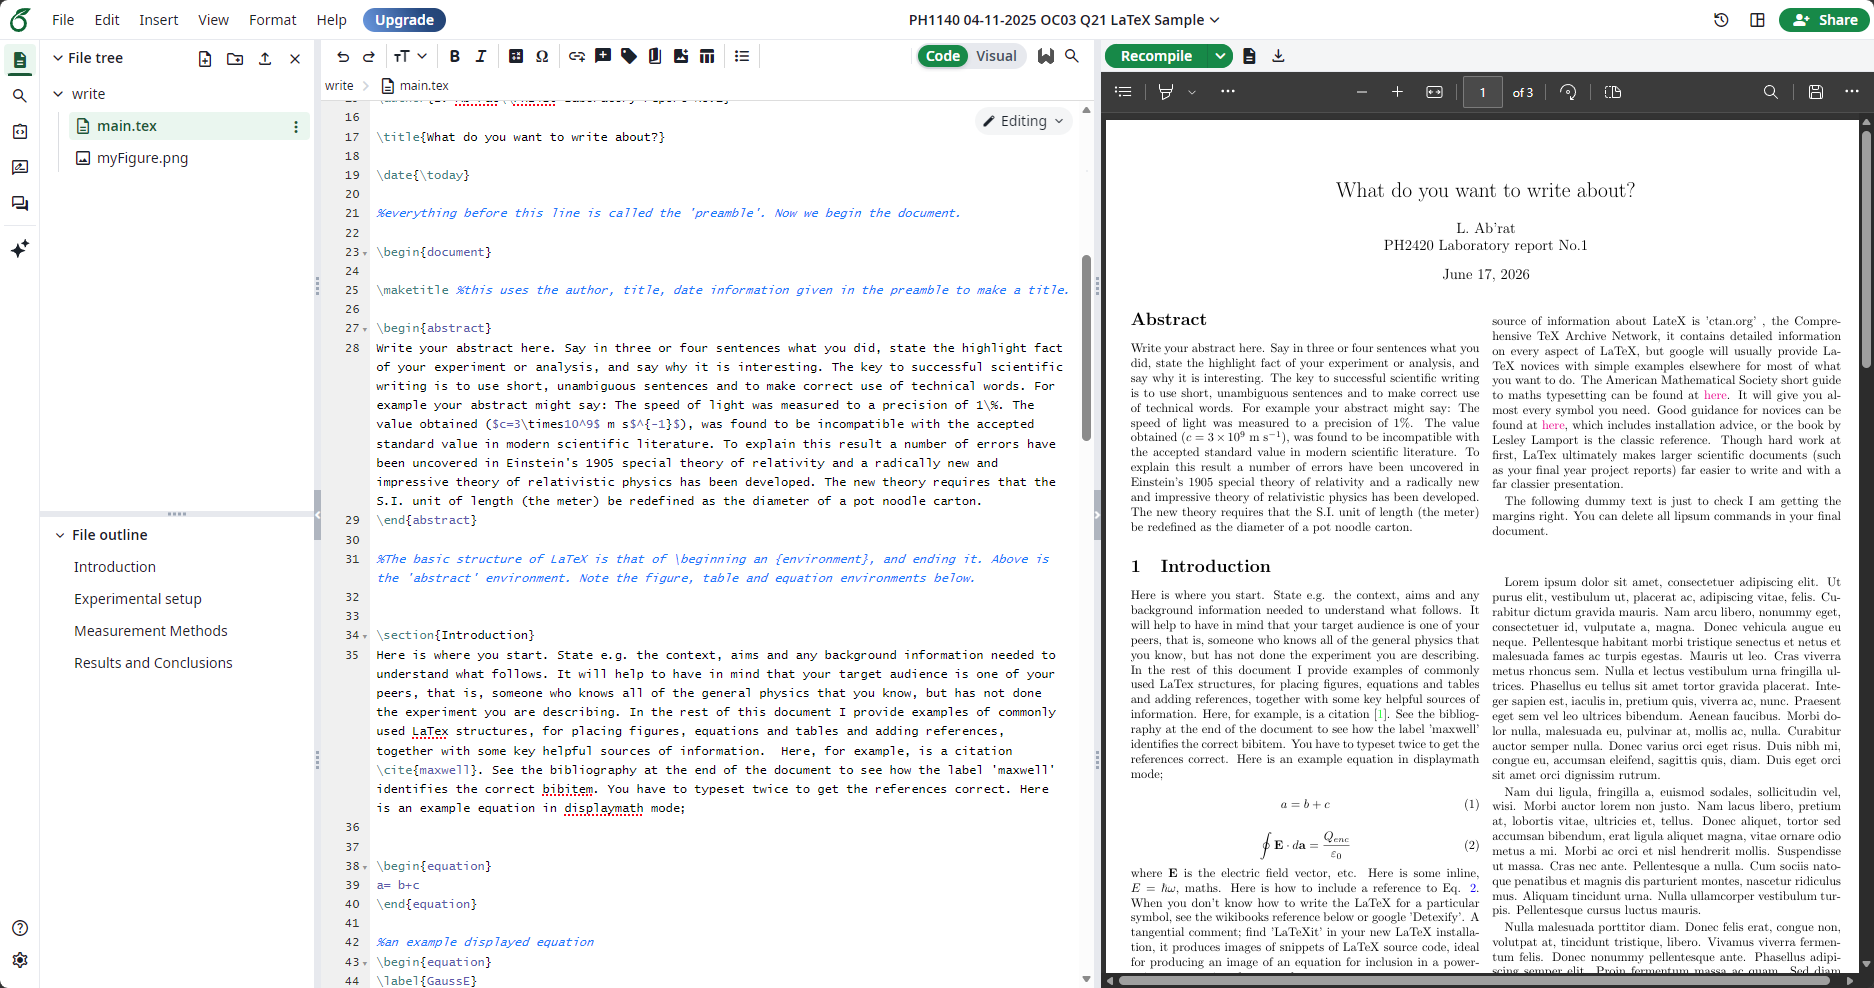
\includegraphics[width=0.75\textwidth, alt={The Overleaf Editor has two main panels for the text editor and PDF viewer, with a sidebar for files and the docuemnt outline. Tools are located on an upper navigation bar.}]{overleaf-editor}
  \caption{The \textit{Overleaf} Editor}
  \label{fig:ovlf-ed}
\end{figure}

\textit{Overleaf} will automatically create a \verb|main.tex| file which you can view in the file tree on the far left. The content of your file is visible in the central editor and the compiled PDF document to the far right (see Figure~\ref{fig:ovlf-ed}). Any files that need to be included in the project must be added to the file tree, which acts as a folder for the project. This will make more sense later once you begin to learn how to make and edit \LaTeX\ files.

Helpfully, \textit{Overleaf} comes with lots of features built-in -- such as auto-compiling and code corrections and completion. The auto-compiling feature means that you will not have to worry about compiling your document, and every change you make is updated in (close to) real-time in the document preview.

Another useful feature is the word counter, which is accessible through the file menu in the top navigation bar of the editor. It also supports standard keyboard shortcuts for italics and boldface.

After compiling your document, you can submit it by clicking the download icon (\raisebox{-0.2em}{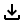
\includegraphics[height=1em,alt={Dowload PDF}]{download}}) next to the `Recompile' button to save your PDF file. Then, simply upload your PDF file to the Moodle submission box. Do not share the project or try to submit it directly from \textit{Overleaf}.

Make sure that you check the log (\raisebox{-0.2em}{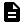
\includegraphics[height=1em,alt={View logs}]{description}}) for any errors before downloading your PDF file -- you may not realise that your code has not worked!

{
  \scriptsize
  \textsc{Note} that \textit{Overleaf} does have paid plans which allow access to more features and compile time, alternatives include \href{https://papeeria.com/}{\textit{Papeeria}} and \href{https://cocalc.com/features/latex-editor}{\textit{CoCalc}}, although their features and pricing plans vary. \textbf{It is not advisable to pay for any \LaTeX\ software.}
}

\subsection{For Desktop}
It is recommended that you use \textit{Overleaf} for all of your \LaTeX\ needs. However, you may run out of compile time when working with big projects, in which case you will not be able to produce PDF files without paying for a plan. This is because you are using their servers to edit and compile your document.

To avoid paying, you can use a desktop distribution of \LaTeX. There are three major distributions to use: \href{https://miktex.org/}{\MiKTeX} and \href{https://www.tug.org/texlive/}{\TeXLive} for \textit{Microsoft Windows}, and \href{https://www.tug.org/mactex/}{Mac\TeX} for \macOS. I recommend using \MiKTeX\ if you use \textit{Microsoft Windows}, which was used to typeset this manual with the \pdfLaTeX\ engine.

More information about these distributions can be found on their websites, and most of them come packaged with the \href{https://tug.org/texworks/}{\TeX works} editor which supports with creating documents as the engines themselves are command line programs with no graphical interfaces.

\section{Syntax}
\LaTeX\ is a language of commands and text, with the commands used to style the text. Any and all text outside of commands is written directly to the output PDF file, with the engine reading (`parsing') through the input \verb|.tex| file from top to bottom to compile a document.

Every command has the same format:
\begin{minted}[numbers=none]{latex}
\command[<options>]{<argument>}
\end{minted}
with two inputs, a main argument (text to be styled) and options which change the way the command acts.

Note that the main argument changes in use, with some commands using it as a required optional parameter instead of text. Commands can be nested by passing them as arguments, and can also be used within options. To add another curveball, some commands do not accept arguments at all! This will all make more sense when you are introduced to some real commands in the next chapter.

\chapter{Writing Reports}
This chapter aims to introduce you to \LaTeX\ coding and support you in writing your first report. After that, you will be introduced to more efficient workflows thanks to packages.

There are many different ways to write \LaTeX\ documents and this guide focuses on core methods rather than the ``correct'' way of doing things, which are matters of taste and not something to be greatly concerned about.

\section{Getting Started}
Begin by opening the \verb|main.tex| file, this is where commands are read from and the heart of your document.

Every \LaTeX\ document starts with one command:
\begin{minted}[numbers=none]{latex}
\documentclass{article}
\end{minted}
for a report, the document class is \textsf{article}, although note that this changes for different types of document (such as for the presentations later...).

We can give the compiler more information about our document, such as the page layout and size, by providing options within square brackets before the document type in braces (\mintinline{latex}{{}}):
\begin{minted}[numbers=none]{latex}
\documentclass[a4paper,twocolumn,twoside]{article}
\end{minted}
here, a two-sided A4 page layout has been selected with two text columns, using the default font size of \qty{10}{points} -- the preferred formatting for first-year reports; as this part will mostly be given to you in report style guides, do not worry about familiarising yourself with all the available options.

Next, we define some information about the file that will be used to create a document title later:
\begin{minted}{latex}
\title{Some Experiment}
\author{L. Ab'rat\\Royal Holloway, University of London}
\date{\today}
\end{minted}
the three commands here define the title, author, and date of the document -- as you may well have guessed. Note that the compiler reads everything in the braces as \LaTeX\ code, so you can pass commands like \mintinline{latex}{\today} for today's date and \mintinline{latex}{\\ } for a new line.

Combined with the document class, these lines make up what is called the `preamble' of the document. In general, the preamble controls the styling of the document without outputting any text. We shall come back to this later with packages.

Finally, we get to the main bulk of a \LaTeX\ file: writing words to the page! The written part of the document is defined within the handily titled `document' environment:
\begin{minted}{latex}
\begin{document}
\maketitle

... % Your document text goes here
\end{document}
\end{minted}
where \mintinline{latex}{%} begins a comment which is not written to the document. The \mintinline{latex}{\maketitle} command uses the information from the preamble to create a title for the document.

An environment can be thought of as a block of content and we will see more examples later with equations and tables. They always have this form, with a \mintinline{latex}{\begin} and an \mintinline{latex}{\end} command stating the type of environment.

Inside the document environment, all text apart from commands (and comments) gets written to the output PDF file.

Now is a good time to test what you have learned so far, try typing the following code into your \verb|main.tex| file and compiling it:
\begin{minted}{latex}
\documentclass[a4paper,twocolumn,twoside]{article}

\title{Learning LaTeX Sample File}
\author{L. Ab'rat\\Royal Holloway, University of London}
\date{\today}

\begin{document}
\maketitle

Hello World!
\end{document}
\end{minted}
check back over these commands as you type, do you understand what they do? Now is your opportunity to test your new-found knowledge and look up anything you do not understand. The internet is a fantastic tool for any coding project, and \LaTeX\ is no different!

\section{Basic Formatting}
Everyone who deals with code knows that there are two types of commands: ones which are for specific use cases, and those that apply in \textit{all} situations. The next sections focus on commands you \textit{really} should know and how to use them.

\subsection{Font Styling}
The very basics of formatting are \textit{italics}, \textbf{boldface}, and \underline{underlining}. By far the most useful is italics, although you can see how all of them are achieved below:
\begin{minted}{latex}
This is normal text. \textit{Followed by some in italics}, \textbf{and then in boldface}.

\textit{\textbf{Why not both?}} \underline{Or underlined?}

\textit{Or adding \emph{emphasis} to text already in italics?}

The options are limitless!
\end{minted}
note that more than one type of formatting can be achieved by nesting commands. The \mintinline{latex}{\emph} command is more general than \mintinline{latex}{\textit}, and would ordinarily act in the same way. However, in the example above, it produces upright text within italicised text (\textit{something like \emph{this}!}).

You can denote computer software, such as \textit{Python} programs and libraries, using the \mintinline{latex}{\verb} command:
\begin{minted}[numbers=none]{latex}
\verb|program|
\end{minted}
notice that it uses pipes (\mintinline{latex}{|...|}) instead of braces. This command produces the output in typewriter font: \verb|program|.

\subsection{Sectioning}
Every report is made up of sections, you will have been introduced to them already, but now you need to title them in your document. This is done with the \mintinline{latex}{\section} command:
\begin{minted}{latex}
\section{Introduction}

\subsection{The Science}

\begin{abstract}
... % Abstracts are a bit different, this bit should really be above the introduction!
\end{abstract}
\end{minted}
with the title of the section given inside the braces. Until another section command is given, all text and commands following a section command belong to that section -- with no closing command. Subsections follow the same rules, just using the \mintinline{latex}{\subsection} command instead. Note that subsections are very rarely used in undergraduate reports as there is often not enough to write about!

Every section and subsection is numbered, with subsections numbered with a dot following their section number.

Abstracts are such an important part of reports that they have a dedicated environment (the \mintinline{latex}{abstract}), which comes without the standard section numbering.

\subsection{Creating Tables}\label{sec:tables}
The first complicated environment is the \mintinline{latex}{table}. Instead of breaking down each command right away, let us first see what a complete table looks like in practice:
\begin{minted}{latex}
\begin{table}
  \centering
  \caption{The current and voltage characteristics of different element samples.}
  \begin{tabular}{ l l l }
    Element & Voltage, $V$ / V & Current, $I$ / A \\
    \hline
    H       & 1.0 $\pm$ 0.1    & 2.0 $\pm$ 0.1    \\
    He      & 4.0              & 5.0              \\
    Li      & 7.0              & 8.0              \\
    Na      & 10 $\pm$ 1       & 11 $\pm$ 1       \\
    \hline
  \end{tabular}
  \label{tab:iv-elem}
\end{table}
\end{minted}
\begin{table}[h!]
  \begin{mdframed}
    \centering
    \caption{The current and voltage characteristics of different element samples.}
    \begin{tabular}{ l l l }
      Element & Voltage, $V$ / V & Current, $I$ / A \\
      \hline
      H       & 1.0 $\pm$ 0.1    & 2.0 $\pm$ 0.1    \\
      He      & 4.0              & 5.0              \\
      Li      & 7.0              & 8.0              \\
      Na      & 10 $\pm$ 1       & 11 $\pm$ 1       \\
      \hline
    \end{tabular}
    \label{tab:iv-elem}
  \end{mdframed}
\end{table}

Breaking down each command:
\begin{itemize}
  \item \mintinline{latex}{\begin{table}...\end{table}} designates the environment for tables;
  \item \mintinline{latex}{\centering} centers the environment on the page;
  \item \mintinline{latex}{\caption} labels your table, make sure this is descriptive so people understand the contents of your table;
  \item \mintinline{latex}{\begin{tabular}...\end{tabular}} codes for the table itself -- we will explore this more after this brief overview; and
  \item \mintinline{latex}{\label} allows you to reference the table (number~\ref{tab:iv-elem}) within your text using the \mintinline{latex}{Table~\ref{tab:iv-elem}} format (see Subsection~\ref{sec:ref}).
\end{itemize}

The \mintinline{latex}{tabular} environment is the hardest part of the table setup, but also the most important! We begin by stating the column format as an extra argument, the text alignment for each column is given with the column separator:
\begin{minted}{latex}
\begin{tabular}{ l l l } % 3 columns of left aligned text with no column separators
\begin{tabular}{|c|c|c|c|} % 4 columns of centred text with lines either side of each column
\begin{tabular}{||r|c||} % 2 columns (right- and centre-aligned) separated by a single line, with a double line outer border.
\end{minted}
we can then use \mintinline{latex}{\hline} to add lines between rows.

The content of each row is then defined by separating each cell with an ampersand (\mintinline{latex}{&}) and ending with a new line (\mintinline{latex}{\\ }). Simple, right?

If, like me, you find this tedious -- worry not! You can use \url[https://]{www.latex-tables.com} to generate table code visually, it even has support for \textit{Microsoft Excel} spreadsheets, they \textit{really} have you covered...

The final thing you may notice is the dollar signs (\mintinline{latex}{$...$}), these signify mathematics which we will cover in Section~\ref{sec:maths} (aptly called \textit{Typesetting Mathematics}).

Note also that you do not need to space things out as in the example, this just makes it easier to read your code!

\subsection{Inserting Images}\label{sec:figures}
Images have been left towards the end of this \textit{Basic Formatting} section as they require a package -- an extra set of predefined commands which we can grab from the internet. Go ahead and add this line to your preamble otherwise the next bit will not work, all will be explained later:
\begin{minted}[numbers=none]{latex}
\usepackage{graphicx}
\end{minted}

Recalling the code from the \textit{Tables} subsection, I will now give an example of an image:
\begin{minted}{latex}
\begin{figure}
  \centering
  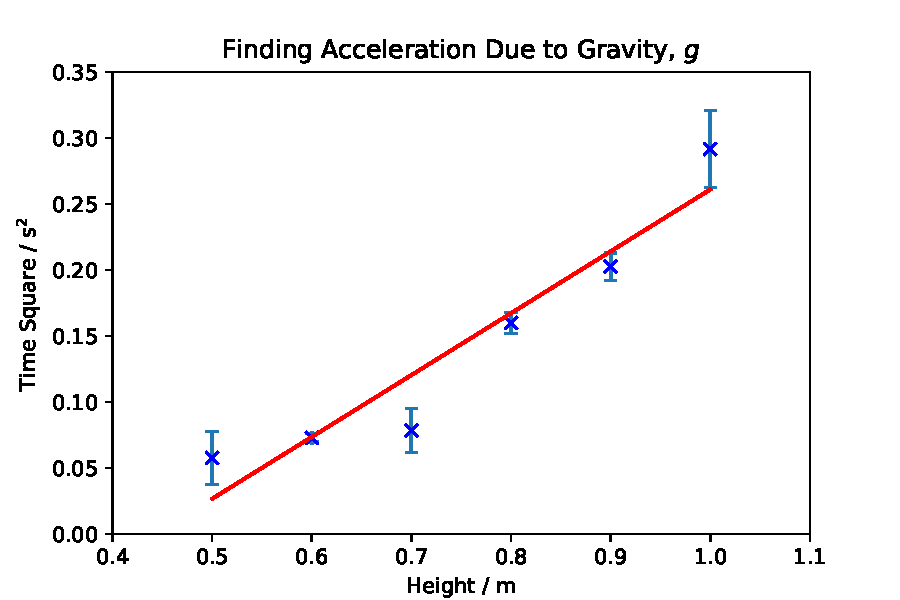
\includegraphics[width=0.75\columnwidth]{figure} % This is too small for this document...
  \caption{A plot of time squared against height to determine $g$.}
  \label{fig:g-calc}
\end{figure}
\end{minted}
\begin{figure}[h!]
  \begin{mdframed}
    \centering
    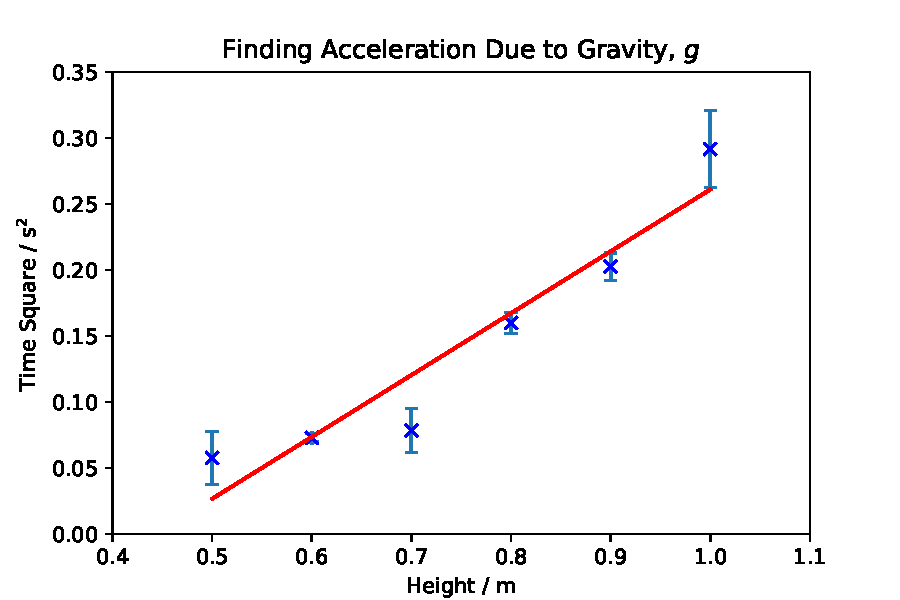
\includegraphics[width=0.75\columnwidth,alt={A plot of time square against height in order to determine the acceleration due to gravity. The image is used for illustrative purposes.}]{figure}
    \caption{A plot of time squared against height to determine $g$.}
    \label{fig:g-calc}
  \end{mdframed}
\end{figure}

You will most likely spot some similarities (and differences!) here:
\begin{itemize}
  \item \mintinline{latex}{\begin{figure}...\end{figure}} designates the environment for figures -- images, plots, etc.; and
  \item \mintinline{latex}{\includegraphics} inserts your image into the document.
\end{itemize}

Most of the heavy-lifting is being done when we `include the graphics.' The argument is the name of the file being inserted, in this case \verb|figure.pdf| -- the file extension \verb|.pdf| is not needed when file names are unique. It is recommended that you insert PDF files for maximum support, however most image files will also work. You will need to add your file for inserting into the file tree (in \textit{Overleaf}) or have it in the same directory as \verb|main.tex|.

In the options of \mintinline{latex}{\includegraphics}, a width has been passed. Most of the time you will want figures to be a full column wide as the text of plots should be the same size as body text. The \mintinline{latex}{\columnwidth} command is used to get the width of the current text column and a decimal multiple can be used for fractional widths.

Finally, notice that the caption has been placed below the figure instead of above. This is because we scan (or read) images differently to tables and text.

\subsection{Cross Referencing}\label{sec:ref}
To reference an object in your \LaTeX\ document, you first need to label the object. Standard objects to label include tables, figures, sections, and equations -- of which the first two should \textit{always} be labelled. To add a label, use the \mintinline{latex}{\label} command:
\begin{minted}{latex}
\section{Method}\label{sec:method} % Labelling a section

\begin{table}
...
\label{tab:table}
\end{table}

\begin{figure}
...
\label{fig:figure}
\end{figure}
% Tables and figures must always be labelled after their content

\label{eq:equation} % The label for an equation - we will see this in use later
\end{minted}
make sure that you use descriptive labels as this will make it easier for you to remember them later!

To reference a labelled object use the \mintinline{latex}{\ref} command:
\begin{minted}{latex}
My Method is Section~\ref{sec:method}.

From the data in Table~\ref{tab:table}, we see that...

See the plot in Figure~\ref{fig:figure} and Equation~\ref{eq:equation} for...
\end{minted}
these phrases have been chosen carefully to specifically name the sections and figures being referenced -- the command only produces a linked number so it helps to add context. The tilde (\mintinline{latex}{~}) is used to ensure that the word and number are not separated across lines, improving readability.

  {
    \scriptsize
    \textsc{Note} that if you are using a desktop distribution, you will often need to compile documents twice if they contain cross references as \LaTeX\ engines update an index file \textit{after} compiling documents with labels.
  }

\section{Typesetting Mathematics}\label{sec:maths}
Mathematics is essential to communicate physics in reports, and luckily \LaTeX\ was designed with it in mind so much so that it is now the most used mathematics typesetting engine across the globe. In this section we will explore how to produce beautiful equations like
\begin{equation}\label{eq:schro}
  -\frac{\hbar^2}{2m}\dv[2]{\psi(x)}{x}+V(x)\psi(x)=E\psi(x)\, ,
\end{equation}
the time-independent 1D Schr\"{o}dinger equation.

\subsection{Mathematics Modes}
By default, mathematical commands cannot be used within a document, you first need to enter a mathematics mode which supports them. There are several different types with varying use cases:
\begin{minted}{latex}
\begin{equation}\label{eq:equation}
...
\end{equation}

This text contains an equation: $...$, and another: \(...\).
\end{minted}
the first pair of commands (\mintinline{latex}{\begin{equation}...\end{equation}}) denote the equation environment (display mode), which produces mathematical expressions on their own numbered line. Notice that this environment can be labelled for referencing, as equations are numbered.

To write mathematics within text, inline mathematics mode can be accessed using dollar signs or the bracket (\mintinline{latex}{\(...\)}) commands. It is generally preferred to use brackets over dollar signs as error messages are easier to debug, however, both are fine.

The inline mode was used in the table and figure examples from Sections~\ref{sec:tables} and~\ref{sec:figures} to include symbols and variables.

It is important to note that mathematics modes do not preserve spaces, so you can space out your mathematics however you choose within your code and it will always be rendered the same!

I will finish this subsection with an aside on how to naturally include equations within reports, for which the standard is something like this (I will define the commands used later, for now only the form is important!):
\begin{minted}{latex}
The quadratic formula is
\begin{equation}\label{eq:quad}
  x = \frac{-b \pm \sqrt{b^2 - 4ac}}{2a}\, ,
\end{equation}
where $x$ is the variable of the equation $ax^2 + bx + c = 0$.
\end{minted}
\begin{mdframed}
  The quadratic formula is
  \begin{equation}\label{eq:quad}
    x = \frac{-b \pm \sqrt{b^2 - 4ac}}{2a}\, ,
  \end{equation}
  where $x$ is the variable of the equation $ax^2 + bx + c = 0$.
\end{mdframed}

Notice that the equation is included within a sentence which gives definitions for all of the variables. In general, equations should not follow a colon and should end with a comma or a full stop (after a thin space, \mintinline{latex}{\, ,} or \mintinline{latex}{\, .}).

\subsection{Basic Commands}
There are so many different mathematics-based commands that to try to list them all would be a pointless exercise, instead I will try to list the most commonly used commands and list some more for reference at the back of this manual -- in Appendix~\ref{chap:matsymb}.

The symbols on your keyboard mostly act as you would expect; a plus (+) codes for a plus sign, the 0 key adds a zero symbol, etc. So we shall start with multiplication and division:
\begin{minted}{latex}
3 \times 4 = 3 + 3 + 3 + 3 = 12
\frac{12}{4} = 3
(12 \div 3) - 1 = 3
\end{minted}
\begin{mdframed}
  $
    \displaystyle
    3 \times 4 = 3 + 3 + 3 + 3 = 12 \\[1em]
    \frac{12}{4} = 3 \\[1em]
    (12 \divisionsymbol 3) - 1 = 3
  $
\end{mdframed}
{
  \scriptsize
  \textsc{Note} that the code above does not give this exact result and is dependent on the environment used. This applies for all code in this section.
}

Ordinary multiplication uses the \mintinline{latex}{\times} command, whilst division makes use of either the \mintinline{latex}{\frac} (fraction) or \mintinline{latex}{\div} (division symbol) commands. The fraction command accepts two arguments, one for the numerator and another for the denominator. In the inline mode, fractions are condensed to fit in a line (like this: $\frac{a}{b}$).

Fractions can be used for derivatives, whilst integrals have their own command:
\begin{minted}{latex}
y = x^2
\frac{dy}{dx} = \frac{\mathrm{d}y}{\mathrm{d}x} = \frac{1}{2}x
\int y\,\mathrm{d}x = \frac{1}{3}x^3 + C
\int_{1}^{3} y\,\mathrm{d}x = \frac{26}{3}
\end{minted}
\begin{mdframed}
  $
    \displaystyle
    y = x^2 \\[1em]
    \frac{dy}{dx} = \frac{\mathrm{d}y}{\mathrm{d}x} = \frac{1}{2}x \\[1em]
    \int y\,\mathrm{d}x = \frac{1}{3}x^3 + C \\[1em]
    \int_{1}^{3} y\,\mathrm{d}x = \frac{26}{3}
  $
\end{mdframed}

Wow, that is a lot! To run through each command:
\begin{itemize}
  \item The caret (\mintinline{latex}{^}) and underscore (\mintinline{latex}{_}) symbols are used for upper (superscript) and lower (subscript) indices respectively, braces can be used to raise and lower more than one character;
  \item \mintinline{latex}{\mathrm} uses a roman font, as this is sometimes preferred for the differential `d' -- but this is a matter of taste;
  \item \mintinline{latex}{\int} is the integral sign, with limits added with indices; and
  \item \mintinline{latex}{\,} is a thin space, the correct spacing between the function and differential of an integral.
\end{itemize}

Trigonometric functions each have their own command:
\begin{minted}{latex}
\sin (\pi \mathrm{\ rad}) = 0
\cos 30^{\circ} = \frac{\sqrt{3}}{2}
\tan x = y
x = \arctan y = \tan^{-1} y
\sin^2 x + \cos^2 x = 1
\end{minted}
\begin{mdframed}
  $
    \displaystyle
    \sin (\pi \mathrm{\ rad}) = 0 \\[1em]
    \cos 30^{\circ} = \frac{\sqrt{3}}{2} \\[1em]
    \tan x = y \\[1em]
    x = \arctan y = \tan^{-1} y \\[1em]
    \sin^2 x + \cos^2 x = 1
  $
\end{mdframed}

We will meet the \mintinline{latex}{\text} command later (in \amsmath, Subsection~\ref{sec:AMS}) which should be used here instead of \mintinline{latex}{\mathrm} -- but this command is not natively supported!

The degree sign is achieved by using a superscript circle (\mintinline{latex}{\circ}) as there is not a degree symbol built into \LaTeX.

Square roots, as you might have noticed, use the \mintinline{latex}{\sqrt} command.

It is important to use commands for functions as writing them in text will render them in italics:
\begin{minted}[numbers=none]{latex}
\sin x \text{ vs } sin x % Yuck! These are not the same...
\end{minted}
\begin{mdframed}
  $
    \displaystyle
    \sin x \text{ vs } sin x
  $
\end{mdframed}

Finally, pi is written using a command, which is the standard for all Greek symbols. Simply spell them out after a backslash to render them. Use an uppercase first letter for uppercase symbols:
\begin{minted}{latex}
\alpha, \beta, \gamma, \Gamma
\theta, \vartheta, \phi, \varphi, \epsilon, \varepsilon % What?!
\end{minted}
\begin{mdframed}
  $
    \displaystyle
    \alpha, \beta, \gamma, \Gamma \\[1em]
    \theta, \vartheta, \phi, \varphi, \epsilon, \varepsilon
  $
\end{mdframed}
some Greek symbols have variants, signified with the \mintinline{latex}{\var} prefix. It is a matter of taste which ones you choose to use -- although I personally like the variants better...

The most common notations for vectors and matrices are coded with:
\begin{minted}{latex}
\mathbf{v} = x\mathbf{i} + y\mathbf{j} + z\mathbf{k}
\mathbf{a} \cdot \mathbf{b} = c
\vec{a} \times \vec{b} = \vec{c}
\mathbf{M}^{-1} = \mathbf{M}^{\mathrm{T}} %...for an orthogonal matrix
\end{minted}
\begin{mdframed}
  $
    \displaystyle
    \mathbf{v} = x\mathbf{i} + y\mathbf{j} + z\mathbf{k} \\[1em]
    \mathbf{a} \cdot \mathbf{b} = c \\[1em]
    \vec{a} \times \vec{b} = \vec{c} \\[1em]
    \mathbf{M}^{-1} = \mathbf{M}^{\mathrm{T}}
  $
\end{mdframed}

Vectors and matrices are often written in boldface, which is produced with the \mintinline{latex}{\mathbf} command (instead of \mintinline{latex}{\textbf}). Although, vectors could be written with an overarrow (thanks to \mintinline{latex}{\vec}).

Dot products make use of a single centred dot (\mintinline{latex}{\cdot}) and cross products we are already familiar with due to the multiplication symbol.

Other common mathematical functions are:
\begin{minted}{latex}
\ln e^x = x % Logarithms
\log 10^y = y
\log_2 8 = 3
\lim_{x \to 0} \frac{\sin x}{\sin 2x} = \frac{1}{2} % Limits
\sum_{n=0}^{5} n = 15 % Summations
\end{minted}
\begin{mdframed}
  $
    \displaystyle
    \ln e^x = x \\[1em]
    \log 10^y = y \\[1em]
    \log_2 8 = 3 \\[1em]
    \lim_{x \to 0} \frac{\sin x}{\sin 2x} = \frac{1}{2} \\[1em]
    \sum_{n=0}^{5} n = 15
  $
\end{mdframed}
note the use of the \mintinline{latex}{\to} command to insert the `tends to' symbol.

As a test of your knowledge, try to reproduce this text in \LaTeX :
\begin{mdframed}
  The formula to differentiate a function from first principles is
  \begin{equation}\tag{1}
    \frac{\mathrm{d}y}{\mathrm{d}x}=\lim_{\Delta x \to 0}\left[ \frac{y(x + \Delta x) - y(x)}{\Delta x} \right]\, ,
  \end{equation}
  where $y$ is a function of $x$ and $\Delta x$ is a small change in the $x$ direction. From this, if $f(\alpha)=\sin 2\alpha$, then
  \begin{equation}\tag{2}
    \frac{\mathrm{d}f}{\mathrm{d}\alpha}=2\cos \alpha\, .
  \end{equation}
\end{mdframed}

Do not worry if you cannot remember everything, there are a lot of commands for mathematics and you will never be required to recall them from memory!

You might also want to attempt to typeset the Schr\"{o}dinger equation \eqref{eq:schro} from the opening of this section. Although, you will need h-bar for that ($\hbar$, \mintinline{latex}{\hbar}).

I would recommend reading through the \textit{Packages} section (number \ref{sec:packages}) which provides more examples of mathematics and information about support for more complex typesetting.

\section{Bibliographies and Referencing}
The final part of a report is referencing your work. This is done using the bibliography-citation system where full references are given in a bibliography at the end of your report and cited within the main text.

At the end of your document (still within the \mintinline{latex}{document} environment), add a \linebreak\mintinline{latex}{thebibliography} environment for your references:
\begin{minted}{latex}
\begin{thebibliography}{1}
  \bibitem{hutley:1982} Hutley, M C. \textit{Diffraction Gratings}. Techniques of Physics. London; New York: Academic Press, 1982. ISBN: 978-0-12-362980-7.
\end{thebibliography}
\end{minted}
\looseness=-1 the argument of the environment is the number of references you have in your bibliography. For example, if you have a bibliography with 12 references, use \linebreak\mintinline{latex}{\begin{thebibliography}{12}}. This ensures that references are correctly spaced on the page.

Within the bibliography, citations can be added using the \mintinline{latex}{\bibitem} command, where the argument is a label for that reference. You should give your references in Vancouver format, the standard for most physics writing, online reference generators may be a useful tool for this.

References should be added in the order they are cited, as \LaTeX\ will not order them automatically.

To cite your reference, use the \mintinline{latex}{\cite} command:
\begin{minted}[numbers=none]{latex}
This is calculated using the diffraction grating equation $d\sin \vartheta = n\lambda$ \cite{hutley:1982}.
\end{minted}
here, the label is passed as the argument to identify the reference being cited. You should cite every time you use a reference within your report, placing the citation at the end of the clause or sentence. You can add notes to citations using the square bracket option format, numbers on their own are interpreted as page numbers.

Putting all this together gives the following result (ignoring the title of the bibliography):
\begin{mdframed}
  This is calculated using the diffraction grating equation $d\sin\vartheta=n\lambda$ [1].\\
  ...
  \begingroup
  \renewcommand{\chapter}[2]{}
  \begin{thebibliography}{99}
    \bibitem{hutley:1982} Hutley, M C. \textit{Diffraction Gratings}. Techniques of Physics. London; New York: Academic Press, 1982. ISBN: 978-0-12-362980-7.
  \end{thebibliography}
  \endgroup
\end{mdframed}

Many people choose to automate the referencing process using \BibTeX\ files, you can read more about this in Subsection~\ref{sec:bib}.

\section{Packages}\label{sec:packages}
So far, we have explored the world of \textit{pure} \LaTeX. Many of the things we have discussed can be improved and expanded using packages -- files which define more commands for us to make use of! \textit{Overleaf}, and the desktop distributions I highlighted earlier, come with lots of package files preloaded so we just need to add the \mintinline{latex}{\usepackage} command to the preamble to access their commands:

\begin{minted}[numbers=none]{latex}
\usepackage[<options>]{<package>}
\end{minted}

The \CTAN\ (\href{https://ctan.org}{ctan.org}) is an archive of a large number of \LaTeX\ packages and hosts documentation for all of the packages I will focus on. It is recommended that you read the documentation for each package you use (\textit{even if you just skim it!}) as there are additional commands I have not mentioned here and there may be specific methods/commands package authors want you to use to achieve different results.

A suggested preamble is provided at the end of this section which has all of the essential packages (and their options) for writing reports.

\subsection{Standard Packages}
These packages are used by everyone writing \LaTeX\ as they add features which are useful for almost every document, meaning you \textit{should} use them in your reports.

\subsubsection{\textsf{geometry}}
The default page layout has a number of issues for reports, which can be addressed with the \textsf{geometry} package:
\begin{minted}[numbers=none]{latex}
\usepackage[margin=0.70cm,includefoot]{geometry}
\end{minted}

This sets the page margins to \qty{0.7}{\cm} whilst still leaving space for page numbering in the footer, removing the unnecessarily large margins from the document.

Note that this package also supports page sizing, which should not be combined with a page size option in the document class.

\subsubsection{\textsf{graphicx}}
By default \LaTeX\ does not support adding graphics to documents, \textsf{graphicx} enables support for this and is what was used in Subsection~\ref{sec:figures} with the \mintinline{latex}{\includegraphics} command.

You can add PDF, PNG, and JPG files to your documents and resize them with the \option{width}, \option{height}, and \option{scale} options -- only specify one of these options per graphic otherwise you will get stretching. PDF is the preferred file format as it imports text natively into documents.

\subsubsection{\texorpdfstring{\amsmath}{AMSmath}}\label{sec:AMS}
The American Mathematical Society (\AMS) has produced two packages which extend the mathematics capabilities of \LaTeX: \textsf{amsmath} and \textsf{amssymb}. Both packages should be loaded together:
\begin{minted}[numbers=none]{latex}
\usepackage{amsmath,amssymb}
\end{minted}

Key functionalities added include:
\begin{itemize}
  \item The \mintinline{latex}{align}, \mintinline{latex}{split}, and \mintinline{latex}{cases} environments;
  \item dynamic bracket (and delimiter) sizing with \mintinline{latex}{\left} and \mintinline{latex}{\right};
  \item \mintinline{latex}{\text} for writing body text inside mathematical modes whilst preserving spaces;
  \item \mintinline{latex}{\eqref} for better equations referencing;
  \item multiple integrals and closed integral symbols;
  \item improved support for matrices; and
  \item fonts for additional symbols.
\end{itemize}

The environments are the largest addition from this list, and we shall start by examining them closer:
\begin{minted}{latex}
\begin{align}
  A & = \pi r^2           \\
    & = \pi \frac{d^2}{4}
\end{align}
\end{minted}
\begin{mdframed}
  \vspace{-1em}
  \begin{align}
    A & = \pi r^2           \\
      & = \pi \frac{d^2}{4}
  \end{align}
\end{mdframed}
the \mintinline{latex}{align} environment automatically enters (display) mathematics mode (so does not require the \mintinline{latex}{equation} environment) and is used to align parts of equations across lines at the ampersand (\mintinline{latex}{&}) character. You can align equations at multiple points by using more than one ampersand -- just make sure that the same number of ampersands appear on each line!

\begin{minted}{latex}
\begin{equation}\label{eq:cases}
  \begin{cases}
    v = u + at      \\
    v^2 = u^2 + 2as
  \end{cases}
\end{equation}
\end{minted}
\begin{mdframed}
  \begin{equation}
    \begin{cases}
      v = u + at \\
      v^2 = u^2 + 2as
    \end{cases}
  \end{equation}
\end{mdframed}
\mintinline{latex}{cases} is an environment for equations which are linked. In the example above, the two SUVAT equations form a pair of simultaneous equations to solve for $t$ and $s$. This \textit{does} require mathematics mode to work.

The final environment, \mintinline{latex}{split}, works similarly to \mintinline{latex}{align}, but produces a single number instead of one for each line. This is covered below, but again \textit{needs} mathematics mode.

Here is a sample of some of the other features in use:
\begin{minted}[escapeinside=||]{latex}
\begin{equation}\label{eq:area}
  \begin{split}
    A & = \pi r_{\text{of circle}}^2       \\
      & = \pi \left( \frac{d^2}{4} \right)
  \end{split}
\end{equation}
The area of a circle is given by \eqref{eq:area}, whilst the volume of a sphere can be found by using the triple integral
\begin{equation}
  \iiint_|V| r^2 \sin \vartheta\, \mathrm{d}r\, \mathrm{d}\vartheta\, \mathrm{d}\varphi\, ,
\end{equation}
where $r$ is the radius of a sphere defined by the volume $V$ in spherical coordinates.
\end{minted}
\begin{mdframed}
  \begin{equation}\label{eq:area}
    \begin{split}
      A & = \pi r_{\text{of circle}}^2       \\
        & = \pi \left( \frac{d^2}{4} \right)
    \end{split}
  \end{equation}
  The area of a circle is given by \eqref{eq:area}, whilst the volume of a sphere can be found by using the triple integral
  \begin{equation}
    \iiint_V r^2 \sin \vartheta\, \mathrm{d}r\, \mathrm{d}\vartheta\, \mathrm{d}\varphi\, ,
  \end{equation}
  where $r$ is the radius of a sphere defined by the volume $V$ in spherical coordinates.
\end{mdframed}

It is good practice to use the \mintinline{latex}{\left} and \mintinline{latex}{\right} commands for all brackets surrounding commands, as you may not always know how different combinations of commands affect the line height.

Multiple integral symbols are defined up to four levels deep (\mintinline{latex}{\iiiint}), where an additional `\verb|i|' is added at the front of the \mintinline{latex}{\int} command for each additional integral symbol.

Additional symbols added by the \textsf{amssymb} package can be found in Appendix~\ref{chap:matsymb}, alongside example usage of the extended matrix environments.

\subsubsection{\textsf{hyperref}}
You may have noticed the {\color{blue} blue links} in this manual. If you took the time to test out some of the examples yourself, you might also have noticed that this is not how links were styled in your documents.

This is made possible using the \textsf{hyperref} package, which adds styling for links:
\begin{minted}[numbers=none]{latex}
  \usepackage[colorlinks=true,linkcolor=blue,urlcolor=blue]{hyperref}
\end{minted}
this is the preferred options, with coloured links enabled and set to {\color{blue} blue}. The default citation colour of {\color{green} green} is used with this set of options.

Note that setting \option{colorlinks} to \option{false} will show links with coloured frames instead of text.

\subsection{Scientific Packages}
The packages under this section will help you to write about science, they are not as widely used but you will most likely find them very useful.

\subsubsection{\textsf{physics}}
The essential package for physics is, handily, called \textsf{physics}! This package aims to make physics equations easier to typeset, with commands that give shortcuts to much more complicated mathematical command sequences -- allowing for:
\begin{itemize}
  \item Nicer inline fractions;
  \item derivatives and differentials;
  \item operators with automatic bracket resizing;
  \item vector notation; and
  \item bra-ket notation.
\end{itemize}
These features can be accessed as:
\begin{minted}[escapeinside=||]{latex}
Normally fractions text look like this: $\frac{a}{b}$ -- but they could look even nicer, like this: $\flatfrac{a}{b}$!

Derivatives and integrals are a lot easier:
\begin{equation}\label{eq:ez-calculus}
  \dv[2]{y}{x} = \int y^{\prime\prime\prime} \dd{x}
\end{equation}
and even support partial derivatives:
\begin{equation}\label{eq:partials}
  \pdv{x}f(x) = \pdv[1]{f}{x}
\end{equation}

Improvements in operators make things easier to typeset than ever before:
\begin{equation}
  \cos(\frac{\vartheta}{2}) = \pm \sqrt{\frac{1 + \cos \vartheta}{2}}
\end{equation}

The beautiful Gauss' divergence theorem states that
\begin{equation}
  \iiint_|V| \left( \div \vb{F} \right) \dd{V} = \oint_|S| \mathbf{F} \vdot \dd{\vb{S}}\, ,
\end{equation}
however, the quantum state vector is an even more fabulous equation, which says that
\begin{equation}
  \ket{\Psi(t)} = \int \Psi(x,t) \ket{x} \dd{x}\, .
\end{equation}
\end{minted}
\begin{mdframed}
  Normally fractions text look like this: $\frac{a}{b}$ -- but they could look even nicer, like this: $\flatfrac{a}{b}$!

  Derivatives and integrals are a lot easier:
  \begin{equation}\label{eq:ez-calculus}
    \dv[2]{y}{x} = \int y^{\prime\prime\prime} \dd{x}
  \end{equation}
  and even support partial derivatives:
  \begin{equation}\label{eq:partials}
    \pdv{x}f(x) = \pdv[1]{f}{x}
  \end{equation}

  Improvements in operators make things easier to typeset than ever before:
  \begin{equation}
    \cos(\frac{\vartheta}{2}) = \pm \sqrt{\frac{1 + \cos \vartheta}{2}}
  \end{equation}

  The beautiful Gauss' divergence theorem states that
  \begin{equation}
    \iiint_V \left( \div \vb{F} \right) \dd{V} = \oint_S \mathbf{F} \vdot \dd{\vb{S}}\, ,
  \end{equation}
  however, the quantum state vector is an even more fabulous equation, which says that
  \begin{equation}
    \ket{\Psi(t)} = \int \Psi(x,t) \ket{x} \dd{x}\, .
  \end{equation}
\end{mdframed}
note that the \textsf{physics} package redefines the \mintinline{latex}{\div} command, moving the division symbol to a new command called \mintinline{latex}{\divisionsymbol}.

More commands are given in Appendix~\ref{chap:matsymb}.

\subsubsection{\textsf{siunitx}}
Quantities and units are a very important part of physics and come with a large amount of formatting conventions. The \textsf{siunitx} package is designed to support these conventions and prevent us from having to think about them:
\begin{minted}[numbers=none]{latex}
  \usepackage[separate-uncertainty=true]{siunitx}
\end{minted}
where the \option{separate-uncertainty} option styles uncertainties with a plus-minus symbol (using \mintinline{latex}{\pm}).

The package adds the following core commands:
\begin{itemize}
  \item \mintinline{latex}{\num};
  \item \mintinline{latex}{\numlist};
  \item \mintinline{latex}{\numrange};
  \item \mintinline{latex}{\ang};
  \item \mintinline{latex}{\qty};
  \item \mintinline{latex}{\qtylist};
  \item \mintinline{latex}{\qtyrange}; and
  \item \mintinline{latex}{\unit}.
\end{itemize}

To avoid repetitive descriptions, let us instead look at all of these commands in use:
\begin{minted}{latex}
I would like \num{5} sandwiches, and my friend would like \num{5.6e-10} drinks. Yes, these are odd choices with a range of \numrange{5.6e-10}{5}.

I measured the diffraction angle of the purple line to be \ang{12;3;45} using the spectrometer. The line was produced by a bulb with a current of \qty{5(0.1)}{\A}. I measured over a voltage range of \qtyrange{1}{5}{\V} with increments of \qty{1}{V}.

The end results found odd results for \qtylist{1;3;5}{\V}. This may be because of the definition of the ohm (\unit{\ohm}), particularly in the microohm (\unit{\micro\ohm}) range. It could also be because of the limited resolution of the multimeter used below \qty{5 \pm 1}{\micro\ohm}.
\end{minted}
\begin{mdframed}
  I would like \num{5} sandwiches, and my friend would like \num{5.6e-10} drinks. Yes, these are odd choices with a range of \numrange{5.6e-10}{5}.

  I measured the diffraction angle of the purple line to be \ang{12;3;45} using the spectrometer. The line was produced by a bulb with a current of \qty{5(0.1)}{\A}. I measured over a voltage range of \qtyrange{1}{5}{\V} with increments of \qty{1}{V}.

  The end results found odd results for \qtylist{1;3;5}{\V}. This may be because of the definition of the ohm (\unit{\ohm}), particularly in the microohm (\unit{\micro\ohm}) range. It could also be because of the limited resolution of the multimeter used below \qty{5 \pm 1}{\micro\ohm}.
\end{mdframed}
here you can see that the package handles all of the grammatical conventions on our behalf, and accepts uncertainties in a range of formats. Unit prefixes are added by using a prefix command before the unit.

Numbers can be provided with erroneous spaces and a variety of exponent notations (including using `\verb|e|' and `\verb|d|') and the package will output them in a standard format:
\begin{minted}[numbers=none]{latex}
\qty{594 78.92455(5)e7}{\centi\m~\ns^{-1}\per\kg\tothe{2}}
\end{minted}
\begin{mdframed}
  \qty{594 78.92455(5)e7}{\centi\m~\ns^{-1}\per\kg\tothe{2}}
\end{mdframed}
note that negative powers can be achieved through using the \mintinline{latex}{\per} command before a unit or by using a negative sign inside of a power (e.g.\ \mintinline{latex}{\A^{-1}}). Do not use both methods at the same time otherwise strange results will follow (like above!). Use tildes (\mintinline{latex}{~}) between units to ensure proper spacing.

A full list of supported units is provided in the documentation, although you can also type unit symbols directly into the unit argument of \textsf{siunitx} commands.

When using \textsf{siunitx} in conjunction with \textsf{physics}, you need to load them using:
\begin{minted}{latex}
\usepackage[separate-uncertainty=true]{siunitx}
\usepackage{physics}
\AtBeginDocument{\RenewCommandCopy\qty\SI}
\end{minted}
to avoid command clashes.

\subsection{Referencing}\label{sec:bib}
\subsubsection{The \texorpdfstring{\BibTeX\ }{BibTeX }File}
Many people choose to automate the creation of bibliographies and citations using packages. All packages make use of the \BibTeX\ file format (ending with \verb|.bib|), which contains entries formatted like this:
\begin{minted}{bibtex}
@book{hutley_1982,
  address = {London; New York},
  series = {Techniques of Physics},
  title = {Diffraction Gratings},
  ISBN = {978-0-12-362980-7},
  callNumber = {QC417 .H87 1982},
  publisher = {Academic Press},
  author = {Hutley, M C},
  year = {1982},
}
\end{minted}

The first line of the entry contains information about the type of reference material and its label (called a citation key), in this case the reference is for a book and we can cite it using \mintinline[escapeinside=||]{latex}{\cite{hutley|\_|1982}} in the same way as manual bibliographies. Note that you cannot use a colon (\option{:}) within citation keys as this is a reserved character.

Inside the entry are fields which provide information about the reference material that will be used to construct a reference. It is generally advisable to include information about as many fields as possible because you will not always know what fields will be used for each reference.

The fields and material types are usually named as you would expect, although it may help to use a cheat sheet (such as the one at the end of this subsection...).

Here are two more examples of \BibTeX\ entries, which you may find useful:
\begin{minted}{bibtex}
@online{sansonetti_2013,
  location = {Gaithersburg, {MD}},
  title = {Atomic Data for Krypton (Kr)},
  url = {https://physics.nist.gov/PhysRefData/Handbook/Tables/ kryptontable1.htm},
  titleaddon = {{NIST} Physical Measurement Laboratory},
  publisher = {National Institute of Standards and Technology},
  author = {Sansonetti, J E and Martin, W C and Young, S L},
  urldate = {2026-02-17},
  date = {2013},
}

@inreference{kaboth_2024,
  title = {Atomic Spectra Team Project},
  booktitle = {{PH}1140/1150 Scientific Skills},
  publisher = {Royal Holloway, {UoL}},
  author = {Kaboth, Asher},
  date = {2024},
  langid = {english},
}
\end{minted}
note that abbreviations are placed inside braces to avoid them being placed in title case.

Many online reference generators support exporting to \BibTeX, and some online reference material such as LibreTexts even have native `download \BibTeX\ reference' options, so you never have to worry about writing them yourself!

\subsubsection{Using \BibLaTeX}
Now that we know about the \BibTeX file format, how do we use it for referencing? Simple, by using a referencing package.

Whilst there are many different referencing packages, this manual will focus on \BibLaTeX. To start out, let us include it as a package and see it in action:
\begin{minted}[escapeinside=||]{latex}
\usepackage[sorting=none,backend=biber]{biblatex}
\addbibresource{main.bib}

\begin{document}
This is calculated using the diffraction grating equation $d\sin\vartheta=n\lambda$ \cite{hutley|\_|1982}.

\printbibliography
\end{document}
\end{minted}
\begin{mdframed}
  This is calculated using the diffraction grating equation $d\sin\vartheta=n\lambda$ [1].\\
  \dots
  \begingroup
  \renewcommand{\chapter}[2]{}
  \begin{thebibliography}{99}
    \bibitem{hutley_1982} M C Hutley. \textit{Diffraction Gratings}. Techniques of Physics. London; New York: Academic Press, 1982. \textsc{isbn}: 978-0-12-362980-7.
  \end{thebibliography}
  \endgroup
\end{mdframed}
note that the title of the bibliography has again been omitted here.

The \mintinline{latex}{\addbibresource} command tells \BibLaTeX\ what our \BibTeX\ file is (\verb|main.bib| in this case), try to make sure that all of your references are in the same file so that it simplifies this step.

We cite things as usual with the \mintinline{latex}{\cite} command, but then use \mintinline{latex}{\printbibliography} to insert the bibliography. When using packages, bibliographies are `clever' and can sort references in many different way, so there is no need to organise your \BibTeX\ files. The \option{sorting} option controls how references should be sorted, with the \option{none} selection sorting them in the same order as they are cited.

Finally, we passed the \option{backend} option to the package. This tells it what binary to use for \BibTeX\ file processing -- in this case \biber. The reasoning behind this is not important, but it ensures that our references are processed in line with \BibLaTeX's expectations.

  {
    \scriptsize
    \textsc{Note} that if you are using a desktop distribution, there is a specific compile sequence required to correctly handle referencing packages. For \BibLaTeX, you should run engines and binaries in this order: \pdfLaTeX\ $\rightarrow$ \biber\ $\rightarrow$ \pdfLaTeX\ $\rightarrow$ \pdfLaTeX. \biber\ is the binary used by \BibLaTeX\ to index \BibTeX\ files, which is why it is run here. \pdfLaTeX\ is run multiple times to correctly gather and use information from the index. This compile sequence is often preloaded with engines as a `recipe,' but you can still run all these tools separately for the same result. \textit{Overleaf} handles all of this automatically so you will only need to compile once.
  }

\subsubsection{Combining Citations}

If it is necessary to cite more than one reference, the \mintinline{latex}{\cites} command can be used, which follows the same format as the \mintinline{latex}{\cite} command, but with more than one citation:
\begin{minted}[numbers=none,escapeinside=||]{latex}
\cites[25]{hutley|\_|1982}|\color{optioncolor}[2-3]|{kaboth|\_|2024}{sansonetti|\_|2013}
\end{minted}
which produces the following result:
\begin{mdframed}
  This statement has multiple citations [1, p. 25, 2, pp. 2--3, 3]!\\
  \dots
  \begingroup
  \renewcommand{\chapter}[2]{}
  \begin{thebibliography}{99}
    \bibitem{hutley_1982} M C Hutley. \textit{Diffraction Gratings}. Techniques of Physics. London; New York: Academic Press, 1982. \textsc{isbn}: 978-0-12-362980-7.
    \bibitem{kaboth_2024} Asher Kaboth. \textit{Atomic Spectra Team Project}. In: \textit{PH1140/1150 Scientific Skills}. Royal Holloway, UoL, 2024.
    \bibitem{sansonetti_2013} J E Sansonetti, W C Martin and S L Young. \textit{Atomic Data for Krypton (Kr)}. NIST Physical Measurement Laboratory. 2013. \textsc{url}: {\urlstyle{tt}\hypersetup{allcolors=black}\url{https://physics.nist.gov/PhysRefData/Handbook/Tables/%20kryptontable1.htm}} (visited on 02/12/2026).
  \end{thebibliography}
  \endgroup
\end{mdframed}

Each citation has its own options, so you can still pass page numbers and notes for each reference. Note that \BibLaTeX\ does not automatically sort citations so it is important that you put them in the correct order. For Vancouver, this should be the order that each reference is used within the phrase.

The example above also shows how different styles of references are formatted, or at least by default, we will discuss how to improve the formatting in the next section.

\subsubsection{Customising the Bibliography}
You should (hopefully) have noticed that the output above is not quite the same as my manual example above. This is because the default reference style is not Vancouver, and whilst there are many different styles which can be selected in \BibLaTeX, none of them \textit{actually} meet our needs. Unfortunately, this means that we have to input some custom styling in the preamble:
\begin{minted}{latex}
\usepackage[giveninits=true,dateabbrev=false,urldate=long, language=british,sorting=none,backend=biber]{biblatex}
\addbibresource{main.bib}
\DeclareNameFormat{default}{%
  \nameparts{#1}%
  \usebibmacro{name:family-given}
    {\namepartfamily}
    {\namepartgiveni}
    {\namepartprefix}
    {\namepartsuffix}%
  \usebibmacro{name:andothers}%
}
\renewcommand{\bibinitperiod}{}
\DeclareFieldFormat{url}{\textsc{url}\intitlepunct\url{#1},}
\DeclareFieldFormat{urldate}{%
  retrieved \thefield{urlday}\addspace%
  \mkbibmonth{\thefield{urlmonth}}\addspace%
  \thefield{urlyear}\isdot
}
\renewbibmacro{in:}{}
\end{minted}

Try not to worry about what is actually happening here, shortly I will give you a file with this styling so you do not have to type it all out. However, the essence is that it redefines how certain fields are printed to the bibliography, adding characters and changing the order of different elements. Extra options have been provided to \BibLaTeX\ to support this custom styling.

You will never be expected to understand or modify this \LaTeX\ code in an undergraduate degree, which is why it is supplied to you here without explanation!

A useful cheat sheet for all things \BibLaTeX\ and \BibTeX\ is available at \url[https://]{ctan.org/pkg/biblatex-cheatsheet}. It includes all of the reference types and their fields, alongside much more detailed information about the \mintinline{latex}{\cite} command.

I will reiterate that it is always better to give more information than \BibLaTeX\ displays than not enough! References are extremely important and just because a tool is producing them for you does not mean you can simply ignore how they are presented.

\subsection{Recommended Configuration}
A sample preamble is provided at \url[https://]{neoski.uk/files/latex/u-report/preamble.tex} which you can download and use:
\begin{minted}{latex}
\input{preamble}

% Remember to update this!
\title{Some Experiment}
\author{L. Ab'rat\\PH1140 OC03 Laboratory Report}
\date{\today}

\begin{document}
\maketitle

% Start writing here
\end{document}
\end{minted}
just make sure that the \verb|preamble.tex| file is in the same folder as \verb|main.tex|.

For users of \textit{Overleaf}, there is a template available which already has this preloaded alongside a basic document outline for you to start with immediately: \url[https://]{overleaf.com/read/zwqxqvrbgtxw\#a65740}, just click `Make a copy' under the file menu (top left). You could also use the file above by using the `Add file from external URL' option -- just make sure you keep the name of the file the same!

\ \linebreak
\hrule
\ \linebreak

Now you have everything you need to typeset excellent reports! The hard part of actually writing them starts now...

Remember that it is OK to make mistakes and that nobody gets everything right the first time -- report writing is a skill just like any other and over time you will come to perfect this gentle art and blow us all away.

\chapter{Creating Presentations}\label{chap:pres}
\LaTeX\ is a very powerful programming language which can typeset not just reports, but books, articles, letters, and \textit{presentations} -- the focus of this chapter. However, not everyone chooses to typeset presentations in \LaTeX\ as it can be incredibly limiting.

The recommended approach for undergraduates is to use \textit{Microsoft PowerPoint} or alternatives such as \textit{Google Slides}. But learning how to use \LaTeX\ for presentations, and more importantly \textit{why}, is still very useful.

\section{Why Use \LaTeX\ for Presentations?}
There are many advantages to using \LaTeX\ for this use case, with the most cited one being that it takes design worries off of the writer, allowing for focus on the content of presentations -- the most important part.

Software packages designed for creating presentations often try to do too much, and tempt you to use their many built-in slide and text styles. This, on its own, is no bad thing. However, there is a very real risk of detracting from the content of a presentation with an overdesigned slide style (such as in Figure~\ref{fig:pres-comp})!

\begin{figure}
  \centering
  $\vcenter{\hbox{\frame{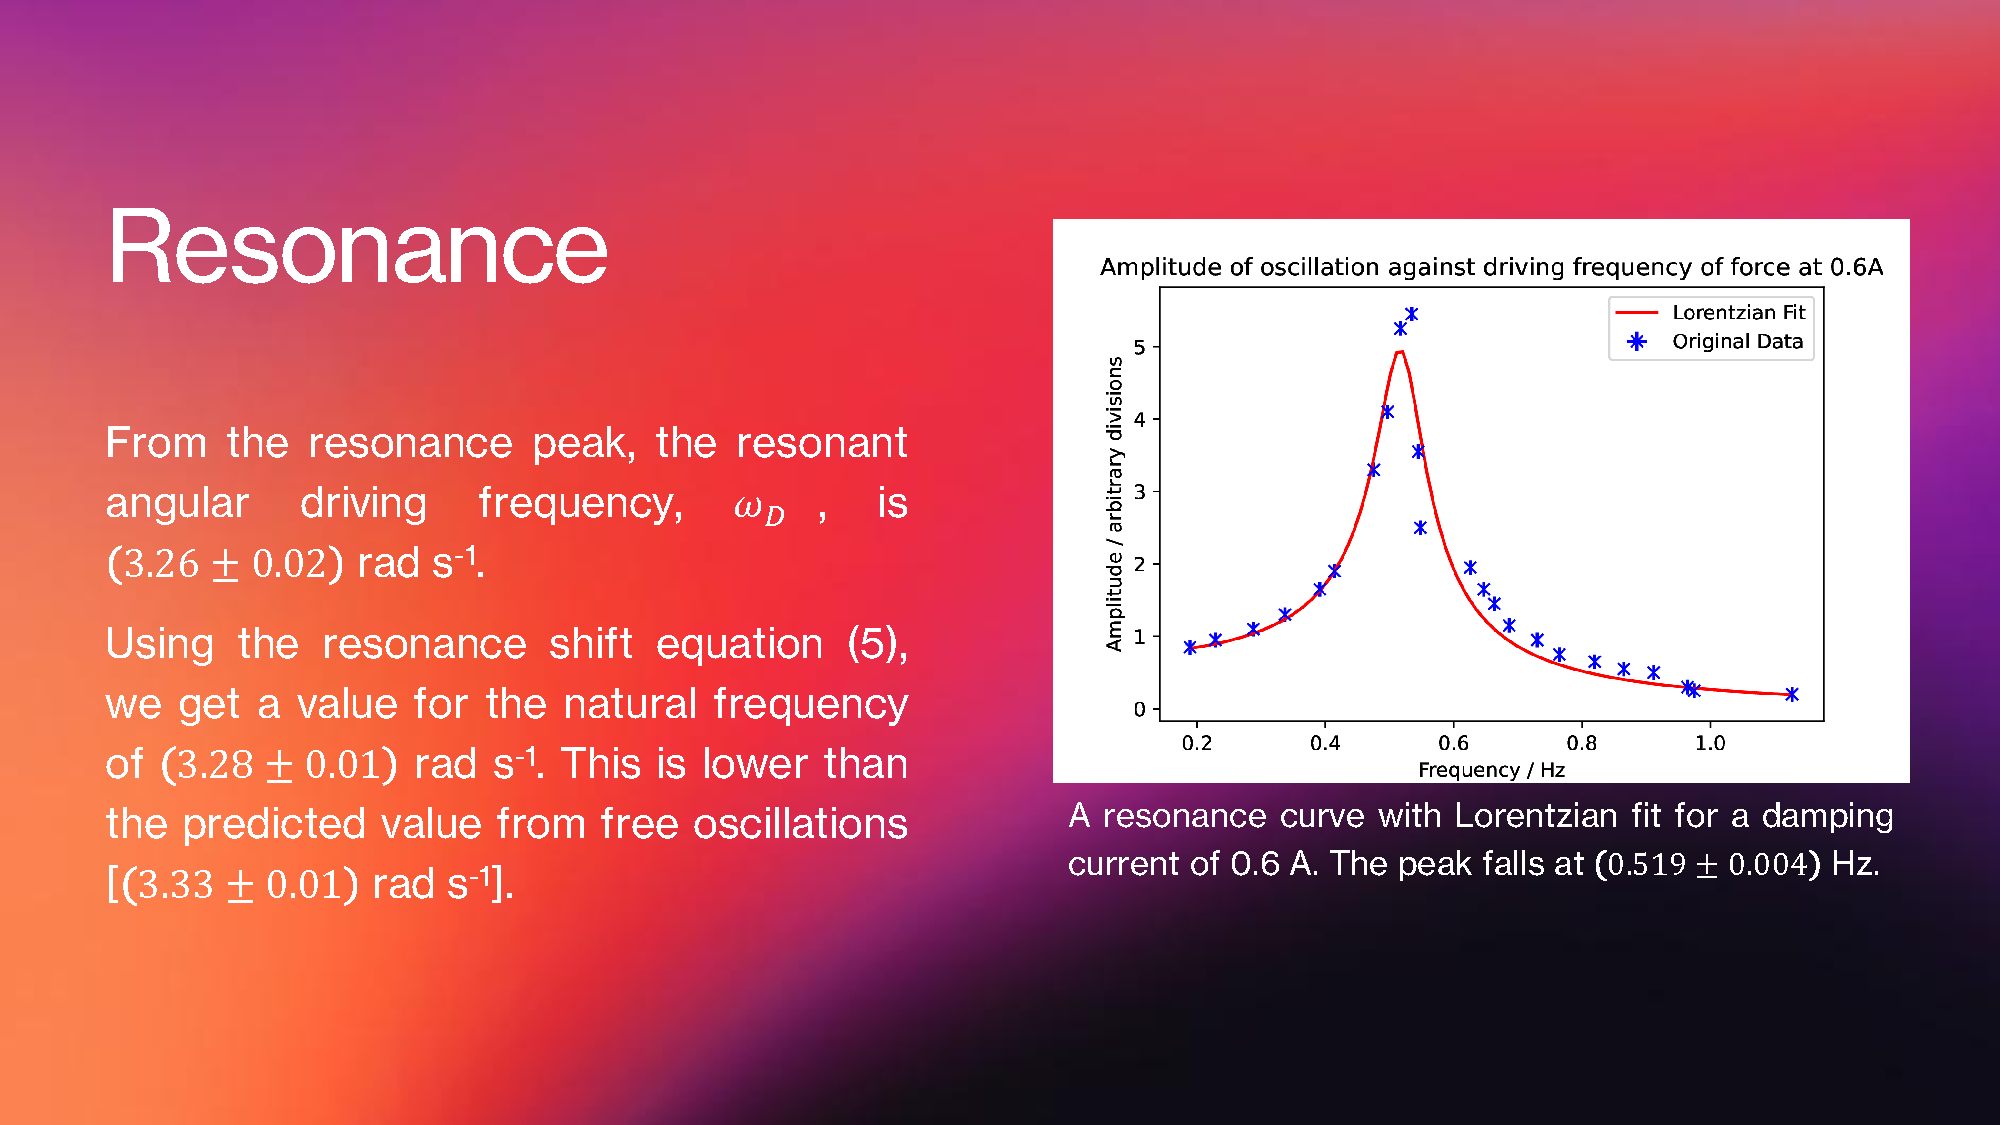
\includegraphics[page=1,width=0.5\textwidth,alt={A Microsoft PowerPoint slide with white text on a vibrant orange, purple, and black image background. A plot takes up the right half of the slide.}]{pres-comp}}}}$
  \hfill
  $\vcenter{\hbox{\frame{\includegraphics[page=3,width=0.45\textwidth,alt={A slide produced in LaTeX with black text on a plain white background. The title and footer have an orange-yellow background. A plot takes up the right half of the slide.}]{pres-comp}}}}$
  \caption{\textsc{Left} An Overdesigned Slide in \textit{Microsoft PowerPoint}, \textsc{Right} A Simple Slide in \LaTeX}
  \label{fig:pres-comp}
\end{figure}

The role of a presentation is as a visual aid for the presenter, it should support the oration delivered and contain key points and graphics. In general, this means that the most simple presentations are the best, as they keep attention on the presenter and their supporting cast of plots, images, and ideas.

But whilst the greatest strength of \LaTeX\ is simplicity, it is also its greatest weakness. You may find that the layout you want to achieve is more difficult to pull off than you first expected, or that the themes are too limited. Of course you can fix many of the problems you will encounter, but it is always worth remembering that \LaTeX\ encourages simplicity for a reason!

Other reasons for typesetting in \LaTeX\ include: native PDF presentations, which are easier to share; extended support for mathematics; and conforming to the style guides of conferences. All of which are important when working professionally, and which tend to make life just that little bit easier.

\section{The \textsf{beamer} Class}\label{sec:beamer}
When writing reports, we used the \textsf{article} document class, however the \textsf{beamer} class is used for presentations -- producing slides instead of pages:
\begin{minted}[numbers=none]{latex}
\documentclass[10pt]{beamer}
\end{minted}

The option here will look pretty similar, specifying a font size of \qty{10}{points} -- the default for this is \qty{11}{points}.

You can continue using all of the same packages with the \textsf{beamer} class, and when writing presentations it is important to remember that the scientific standards still apply! Quantities and units should be correctly formatted and equations produced to exacting specifications -- whether you are typesetting in \LaTeX\ or otherwise...

\begin{samepage}
  Note that the \textsf{geometry}, \textsf{hyperref}, and \textsf{graphicx} packages are loaded by the \textsf{beamer} class itself (or are incompatible!) so should not be included separately to avoid option conflicts. By default, slides have a 4:3 aspect ratio, to switch to a more standard 16:9 ratio pass it as an option when defining the document class:
  \begin{minted}[numbers=none]{latex}
\documentclass[10pt,aspectratio=1609]{beamer}
\end{minted}
  where \option{1609} is interpreted as the ratio 16:09. To change \textsf{hyperref} options, use \option{hyperref}:
  \begin{minted}[numbers=none]{latex}
\documentclass[10pt,hyperref={linkcolor=blue}]{beamer}
\end{minted}

  There are also different document information commands available for presentations:
\end{samepage}
\begin{minted}{latex}
\title{Some Presentation}
\subtitle{A Gripping Account of My Research}
\author{L. Ab'rat}
\institute[RHUL]{Royal Holloway, University of London}
\date{\today}
\end{minted}
here, most of the commands are self-explanatory, with the \mintinline{latex}{\institute} referring to your place of work (Royal Holloway). Square brackets can be used with all of the information commands to provide a shorter version of the content, which is used in the slide footer where space is limited.

You may be presenting as a group, in which case you can use the \mintinline{latex}{\and} command for additional authors:
\begin{minted}[numbers=none]{latex}
\author[Ab'rat \and Skinner]{L. Ab'rat \and N. L. Skinner}
\end{minted}

\subsection{Creating Frames}
\LaTeX\ presentations are based around environments called frames, which take the place of traditional slides. Each frame should be explicitly defined and titled:
\begin{minted}{latex}
\begin{frame}{Title}
  ...
\end{frame}
\end{minted}
where the title is passed as an additional argument. Note that it is possible to produce frames without titles by leaving the argument empty, but this is not generally advisable.

All presentations begin with a title slide, which can be produced by using the \mintinline{latex}{\titlepage} command inside of an empty frame:
\begin{minted}{latex}
\begin{frame}
  \titlepage
\end{frame}
\end{minted}

Try testing things out now with a simple sample presentation:
\begin{minted}{latex}
\documentclass[10pt]{beamer}

\title{Making Presentations}
\subtitle{A Sample LaTeX File}
\author{L. Ab'rat}
\institute[RHUL]{Royal Holloway, University of London}
\date{\today}

\begin{document}

\begin{frame}
  \titlepage
\end{frame}

\begin{frame}{Introduction}
  Hello World!

  Welcome to my presentation...
\end{frame}

\end{document}
\end{minted}

Go ahead and type this code block into a \LaTeX\ file and compile it. Remind yourself of the role of each command and their options. Creating presentations is different to writing reports, so it is important that you understand the similarities and differences in their code. Your presentation should look like this:

\begin{figure*}[h!]
  \centering
  \frame{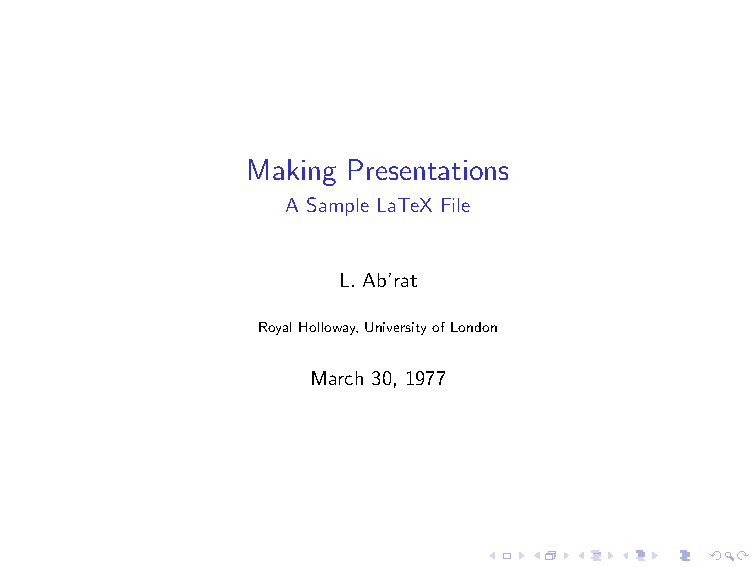
\includegraphics[page=1,width=0.475\textwidth]{pres-ex}}
  \hfill
  \frame{\includegraphics[page=2,width=0.475\textwidth]{pres-ex}}
\end{figure*}

This is your first glimpse of what a \LaTeX\ presentation looks like -- we will make some changes to this in the next subsection.

In the \textsf{beamer} class you can continue to use all of the \LaTeX\ commands you are used to, including inserting figures, tables, and mathematics -- just remember to think about how much space you have on each frame! It is advised that you use no more than 40 words on each frame, with figures, tables, and graphics most effective on their own frames.

\subsection{Themes}
The standard presentation style is plain and functional, but perhaps a bit boring! We can improve this by using themes. There are two different types of theme: presentation themes and colour themes.

\textit{Presentation themes} style the layout of frames, whilst \textit{colour themes} change -- you guessed it -- the colour scheme. To understand what is possible, let us take some time to look at two examples of both in detail using the sample file above.

Themes can be selected in the preamble of documents:
\begin{minted}{latex}
\usetheme{Theme} % Presentation themes are title case
\usecolortheme{colours} % Colour themes are not
\end{minted}

\textsf{Boadilla} is a presentation theme which introduces a footer to frames, providing additional document information on each frame:
\begin{figure*}[h!]
  \centering
  \frame{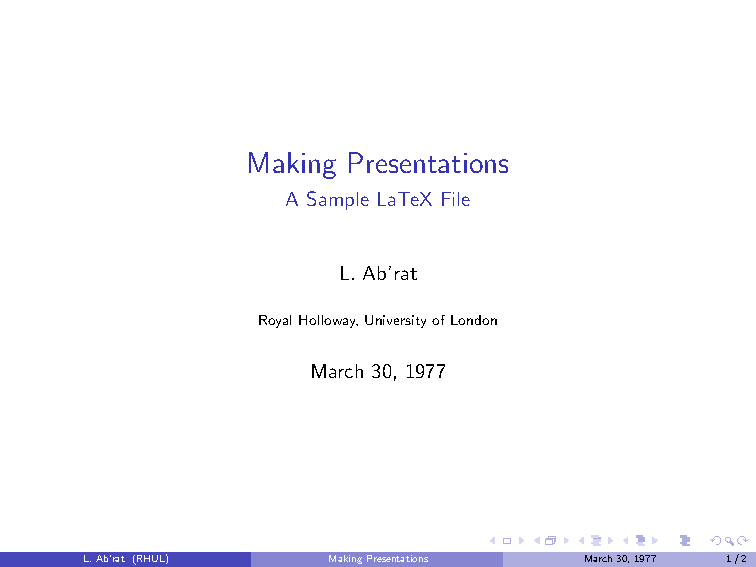
\includegraphics[page=1,width=0.475\textwidth]{pres-themes}}
  \hfill
  \frame{\includegraphics[page=2,width=0.475\textwidth]{pres-themes}}
\end{figure*}

You can use this theme by adding \mintinline{latex}{\usetheme{Boadilla}} to your preamble -- note the capitalisation.

Another presentation theme is \textsf{PaloAlto}, it uses a sidebar instead of a footer:
\begin{figure*}[h!]
  \centering
  \frame{\includegraphics[page=5,width=0.475\textwidth]{pres-themes}}
  \hfill
  \frame{\includegraphics[page=6,width=0.475\textwidth]{pres-themes}}
\end{figure*}

Presentation themes are often named after cities, as these were the locations of important mathematical conferences which had presentation style guides, many of which have been adapted and are now available for anyone to use.

These presentation themes can be combined with colour themes to produce a much larger variety of options. There are 27 presentation themes which can be combined with any one of 15 colour themes, leading to 405 possibilities from just the base themes! You can also specify custom colours and options if you really want unique styles...

For example, \textsf{Boadilla} can be used with the \textsf{crane} colour theme for a bright and vibrant presentation:
\begin{figure*}[h!]
  \centering
  \frame{\includegraphics[page=3,width=0.475\textwidth]{pres-themes}}
  \hfill
  \frame{\includegraphics[page=4,width=0.475\textwidth]{pres-themes}}
\end{figure*}

The \textsf{crane} colour theme can be specified with the \mintinline{latex}{\usecolortheme{crane}} command. In this case the \textsf{Boadilla} presentation theme has also been specified using the command mentioned previously.

It is important to test out theme combinations before using them to make sure that your presentations are readable. For example, the \textsf{PaloAlto} presentation theme does not work well with the \textsf{beaver} colour theme as it uses a white font in the sidebar -- meaning the document title is unreadable!
\begin{figure*}[h!]
  \centering
  \frame{\includegraphics[page=7,width=0.475\textwidth]{pres-themes}}
  \hfill
  \frame{\includegraphics[page=8,width=0.475\textwidth]{pres-themes}}
\end{figure*}

If you do not want to try out all of the theme combinations for yourself, you can view all of the options at \url[https://]{hartwork.org/beamer-theme-matrix}.

Many institutions have custom themes which you must use for your presentations, however undergraduates are normally free to use whatever they think looks best!

\subsection{Writing Notes}
A good presenter is prepared with notes so they know what they are supposed to say. \LaTeX\ presentations have notes built-in so you can do everything in one place instead of having to laboriously hand-write cue cards.

There are a couple of different ways of adding notes to frames, but we will start with the most straightforward:
\begin{minted}{latex}
\begin{frame}{Frame with Notes}
  This is my very important frame contents.
  \note[item]{It really is \textit{very} important!}
  
  Here is a bit more...
  \note[item]{This bit may be aided with the formula $a+b=12$.}
\end{frame}
\end{minted}
this adds notes as a numbered list, placing them on a separate notes page -- which is not normally visible! To show notes pages add the \textsf{beamer} option to your preamble:
\begin{minted}[numbers=none]{latex}
\setbeameroption{show notes}
\end{minted}
which then produces:
\begin{figure*}[h!]
  \centering
  \frame{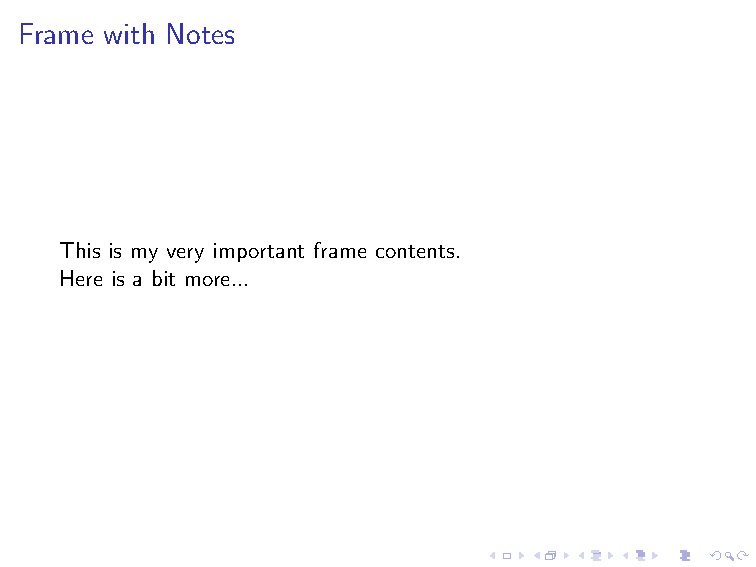
\includegraphics[page=1,width=0.475\textwidth]{pres-notes}}
  \hfill
  \frame{\includegraphics[page=2,width=0.475\textwidth]{pres-notes}}
\end{figure*}

There are a couple of different options for notes pages, which are usually written in the preamble to be enabled as and when required:
\begin{minted}{latex}
% Uncomment each line as needed:
% \setbeameroption{show notes}
% \setbeameroption{show only notes}
% \setbeameroption{show notes on second screen=right}
\end{minted}
the first of these commands we are already familiar with, but there are also options for showing only notes pages (line~3) and displaying both frames and notes side-by-side (line~4), which is particularly useful as it makes both your frame contents and notes easy to see when presenting.

You may also want to write all of your notes in one go instead of line-by-line, for which the \mintinline{latex}{\note} command is again used:
\begin{minted}{latex}
\begin{frame}{Frame with Notes}
  This is my very important frame contents.

  Here is a bit more...

  \note{
    All of my notes can go here, formatted as you would expect with a LaTeX document!

    Leave a space between lines to start a new paragraph.
  }
\end{frame}
\end{minted}
as you might have spotted, notes support all of the standard \LaTeX\ commands. This means you can add mathematics and even apply emphasis to important words and phrases! As an additional word of advice: do not add graphics, figures, and tables to notes pages as your frames will already have them -- just use the side-by-side display option:
\begin{figure*}[h!]
  \centering
  \frame{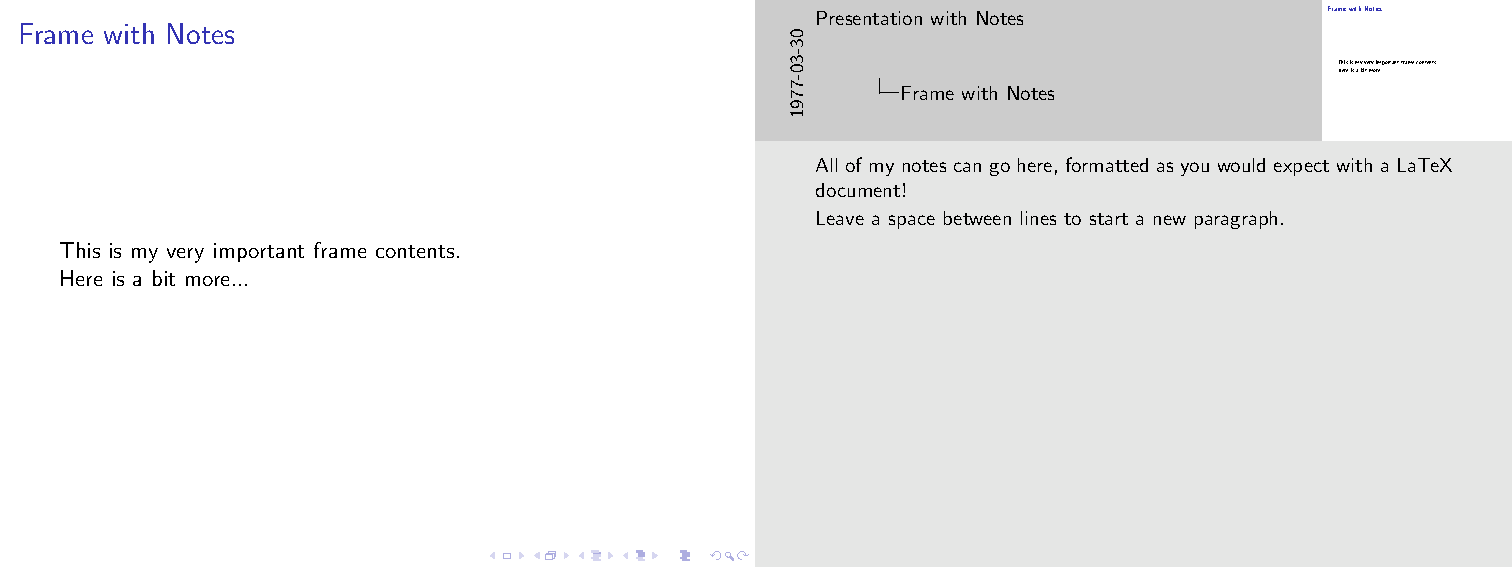
\includegraphics[page=1,width=0.95\textwidth]{pres-notes2}}
\end{figure*}

You can also style the notes pages to better suit your needs and preferences, I cover this in Subsection~\ref{sec:note-sty}.

Finally, if you are giving presentations, you might find that a PDF viewer which displays two documents at the same time will come in handy. A web-based viewer with support for this is available at \url[https://]{beamerviewer.euxane.eu} and also has a timer on the notes page so you know exactly how long you have spoken for. Note that presentations must be in side-by-side mode to show correctly.

\section{Formatting for Speech}
When delivering presentations, our speech often matches with different document structures to what we might use with reports. In general, shorter and more informal phrases are used in speech and it is important to mirror this when writing presentations.

It is also important to highlight key parts of text and formulae on slides and frames to ensure that the audience understands how the presentation matches with your speech.

The next subsections focus on different formatting techniques which are best suited for presentations and how to effectively use them.

\subsection{Lists}\label{sec:lists}
There are two different types of list: bulleted and numbered. \LaTeX\ supports both types and distinguishes between the two by using different environments. Take a look at the following example:
\begin{minted}{latex}
\begin{itemize}
  \item One
  \item Two
  \item Three
\end{itemize}

\begin{enumerate}
  \item One
  \item Two
  \item Three
\end{enumerate}
\end{minted}
\begin{mdframed}
  \begin{itemize}
    \item One
    \item Two
    \item Three
  \end{itemize}

  \begin{enumerate}
    \item One
    \item Two
    \item Three
  \end{enumerate}
\end{mdframed}
the \mintinline{latex}{itemize} environment is used for bulleted lists, whilst \mintinline{latex}{enumerate} is for numbered lists. Each list item starts with an \mintinline{latex}{\item} command, anything that follows this command is indented under that list item -- including environments, allowing for nested lists:
\begin{minted}{latex}
\begin{itemize}
  \item Nested List
        \begin{enumerate}
          \item Nesting lists was shared,
          \item you said it was a \textit{hack},
          \item but Einstein said
                \begin{equation}
                  E = mc^2\, ,
                \end{equation}
                and we never looked \textit{back}!
        \end{enumerate}
  \item The List Continues...
\end{itemize}
\end{minted}
\begin{mdframed}
  \begin{itemize}
    \item Nested List
          \begin{enumerate}
            \item Nesting lists was thought to be a \textit{hack},
            \item but Einstein said
                  \begin{equation}
                    E = mc^2\, ,
                  \end{equation}
                  and we never looked \textit{back}!
          \end{enumerate}
    \item The List Continues...
  \end{itemize}
\end{mdframed}

Lists are very useful for presentations as they are an essential part of speech. You may want to use them for listing methods and equipment.

\subsection{Blocks}
Another part of speech is the \textit{aside}. One topic leads to another and before we know it, a full-blown tangent has led us astray and the original topic is long lost...

Asides can be turned on their head and used in presentations to highlight things which are really important, when explaining equations (for example) it is often helpful to explain why it has that form. In presentations, the \mintinline{latex}{block} environment allows for this kind of highlighting:
\begin{minted}{latex}
\begin{block}{Euler's Formula}
  My calculations used Euler's Formula, which states that
  \begin{equation}
    e^{i\varphi} = \cos\varphi + i\sin\varphi\, ,
  \end{equation}
  where $\varphi$ is the argument of the complex number.
\end{block}
\end{minted}
\begin{mdframed}
  \sffamily
  \sansmath
  \vspace*{-0.8em}
  \begin{block}{Euler's Formula}
    My calculations used Euler's Formula, which states that
    \begin{equation}
      e^{i\varphi} = \cos\varphi + i\sin\varphi\, ,
      \refstepcounter{equation}\tag*{\textsf{(\theequation)}}
    \end{equation}
    where $\mathsf{\varphi}$ is the argument of the complex number.
  \end{block}
  \unsansmath
\end{mdframed}
notice that the block title is passed as an additional argument. The styling of blocks change based on which combination of themes is selected, so they may appear different to this example.

There are different types of blocks available to use, which differ in colour and use. These are:
\begin{itemize}
  \item \mintinline{latex}{block} the default (or generic) style,
  \item \mintinline{latex}{alertblock} for important information,
  \item \mintinline{latex}{exampleblock} for examples,
  \item \mintinline{latex}{theorem} for mathematical theorems,
  \item \mintinline{latex}{definition} for defined mathematical expressions,
  \item \mintinline{latex}{proof} for proofs,
  \item \mintinline{latex}{lemma} for intermediate theorems,
  \item \mintinline{latex}{corollary} for subsequent propositions, and
  \item \mintinline{latex}{example} as an alternative to \mintinline{latex}{exampleblock}.
\end{itemize}
Many of these are for mathematical use and may not be useful in most physics writing. However, you may wish to use \mintinline{latex}{alertblock} and \mintinline{latex}{exampleblock} for other purposes as they are coloured red and green (respectively), offering an opportunity for different types of content.

All blocks which do not finish with `\mintinline{latex}{block}' do not accept title arguments and so have limited use cases.

Note that the block commands are not defined for use with other \LaTeX\ document classes.

\subsection{Labelling Mathematics}\label{sec:label}
Sometimes it helps to annotate equations by labelling expressions, this can be done by using over- and underbraces:
\begin{minted}{latex}
The equation for a mass-spring system is:
\begin{equation}
  \underbrace{m\dv[2]{\mathbf{x}}{t}}_{\text{acceleration}} + \overbrace{k\dv{\mathbf{x}}{t}}^{\text{damping}} = \underbrace{\mathbf{F}(\mathbf{x})}_{\text{force}}\, .
\end{equation}
\end{minted}
\begin{mdframed}
  The equation for a mass-spring system is:
  \begin{equation}\label{eq:mass-spring}
    \underbrace{m\dv[2]{\mathbf{x}}{t}}_{\text{acceleration}} + \overbrace{k\dv{\mathbf{x}}{t}}^{\text{damping}} = \underbrace{\mathbf{F}(\mathbf{x})}_{\text{force}}\, .
  \end{equation}
\end{mdframed}
where text can be added by using super- and subscripts on the \mintinline{latex}{\overbrace} and \mintinline{latex}{\underbrace} commands.

This formatting makes it clear what parts of equations you are referring to and avoids having to describe terms each time you discuss them. The labels are already in mathematics mode, so you can assign terms to easier symbols or show what they cancel to:
\begin{minted}{latex}
The expression
\begin{equation}
  m\underbrace{\dv[2]{\mathbf{x}}{t}}_{\mathbf{a}} + \overbrace{k\dv{\mathbf{x}}{t}}^{=0} = \mathbf{F}(\mathbf{x})\, ,
\end{equation}
can be simplified as
\begin{equation}
  m\mathbf{a} = \mathbf{F}(\mathbf{x})\, .
\end{equation}
\end{minted}
\begin{mdframed}
  The expression
  \begin{equation}
    m\underbrace{\dv[2]{\mathbf{x}}{t}}_{\mathbf{a}} + \overbrace{k\dv{\mathbf{x}}{t}}^{=0} = \mathbf{F}(\mathbf{x})\, ,
  \end{equation}
  can be simplified as
  \begin{equation}
    m\mathbf{a} = \mathbf{F}(\mathbf{x})\, .
  \end{equation}
\end{mdframed}

These examples require \amsmath\ -- an alternative style may be to highlight parts of equations, which is shown in Subsection~\ref{sec:pres-pack}.

\section{Frame Layouts}
Often, you may want to display text alongside figures within the same frame, in which case you may find the following subsections useful -- they contain recommendations for common side-by-side formatting environments.

\subsection{Formatting Columns}\label{sec:col}
By far the easiest way to change the layout of frames is the \mintinline{latex}{columns} environment:
\begin{minted}{latex}
\begin{columns}

  \begin{column}{0.5\textwidth}
    This is column one -- on the left!
  \end{column}

  \begin{column}{0.5\textwidth}
    And now one for the right.
  \end{column}

\end{columns}
\end{minted}

Inside the environment, we use individual \mintinline{latex}{column} environments for each column and pass the required width argument. There is no limit for the number of columns, but it usually advisable to stick with two as things can become crowded very quickly.

I usually recommend adding more space between columns to create a visual break, making frames easier to read. This could be achieved by using column widths of \mintinline{latex}{0.47\textwidth}. For uneven columns, a split of \mintinline{latex}{0.37} to \mintinline{latex}{0.57} (\mintinline{latex}{\textwidth}) should also work pretty well.

Uses of this include displaying text alongside figures, plots, and equations (as seen in Figure~\ref{fig:pres-comp}). Do not include two columns of text on a frame.

\subsection{Figure Environments}\label{sec:subfig}
The \textsf{subcaption} package adds the ability to group multiple figures into one environment. It provides the \mintinline{latex}{\subcaptionbox} command which can be used inside a \mintinline{latex}{figure} environment to create a subfigure:
\begin{minted}{latex}
\begin{figure}
  \centering
  \subcaptionbox{Image A\label{fig:multi-a}} {\includegraphics[width=0.45\textwidth]{a}}
  \subcaptionbox{Image B\label{fig:multi-b}} {\includegraphics[width=0.45\textwidth]{b}}
  \caption{Multiple Figures in One!}
  \label{fig:multi}
\end{figure}
\end{minted}
\begin{figure}[h!]
  \begin{mdframed}
    \centering
    \subcaptionbox{Image A\label{fig:multi-a}}{\includegraphics[artifact,width=0.45\textwidth,actualtext=A]{example-image-a}}
    \subcaptionbox{Image B}{\includegraphics[artifact,width=0.45\textwidth,actualtext=B]{example-image-b}}
    \caption{Multiple Figures in One!}
  \end{mdframed}
\end{figure}
the first argument of the command is for the caption (and label), whilst the second is for the figure itself. Note that to reference the subfigure, you must add the label inside of the caption field (labelling Figure~\ref{fig:multi-a}, for example).

The rest of the figure environment is the same as normal, requiring a separate caption and label for the collection of subfigures.

To create a grid of subfigures, you can add line breaks (\mintinline{latex}{\\ }) between rows of figures. Although take care, as the text size within plots should be the same as body text.

\section{Design and Setup Ideas}
There are a few changes you may want to make to the default \textsf{beamer} setup, I have compiled my favourites below.

\subsection{Packages}\label{sec:pres-pack}
Some packages that work particularly well with presentations are listed below with some recommended use cases. Also see the \textsf{subcaption} package from Subsection~\ref{sec:subfig}.

\subsubsection{\textsf{xcolor}}
One of the most used and abused packages for \LaTeX\ is \textsf{xcolor}, which adds support for a practically infinite array of colours for use within documents. So far, I have avoided mentioning it as colours are very complicated things within scientific writing and something that is hard to get right.

The main problem is accessibility: making sure that colours are readable in a variety of different situations and visually distinct for everyone. You will have already run into this when generating plots for laboratory reports, where the \textit{Python} library \verb|matplotlib| provides an excellent set of default colours specially chosen for people with colourblindness (see Figure~\ref{fig:py-col}).

\begin{figure}[ht]
  \centering
  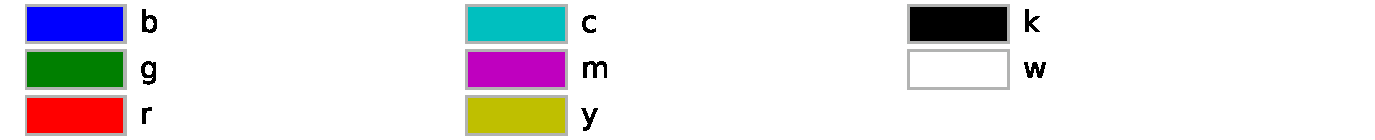
\includegraphics[width=\textwidth,alt={matplotlib offers blue, green, red, cyan, magneta, yellow, black, and white as default colours.}]{py-col}
  \caption{The default colours of \texttt{matplotlib} for \textit{Python}, chosen with accessibility in mind.}
  \label{fig:py-col}
\end{figure}

These complications are why it is important to only use colour where \textit{necessary}. The use case that I will draw attention to here is highlighting, which serves as an alternative to the labelling in Subsection~\ref{sec:label}. In this case, the \mintinline{latex}{\colorbox} command provides what we need:
\begin{minted}{latex}
This is an equation with highlighting:
\begin{equation}
  \oint \vb{E} \vdot \dd{\vb{A}} = \frac{Q}{\colorbox{yellow}{$\varepsilon_0$}}\, .
\end{equation}
\end{minted}
\begin{mdframed}
  This is an equation with highlighting:
  \begin{equation}
    \oint \vb{E} \vdot \dd{\vb{A}} = \frac{Q}{\colorbox{yellow}{$\varepsilon_0$}}\, .
  \end{equation}
\end{mdframed}
where the first argument of the command is the colour and the second is for the highlighted text. Note that \mintinline{latex}{\colorbox} exits the mathematics mode so you will need to enter the inline mathematical mode for the part inside the command.

But, this is just one option, you could also colour the text itself:
\begin{minted}{latex}
Alternatives are just around the corner:
\begin{equation}
  \vb{F}_{\mathrm{L}} = q\left( \textcolor{blue}{\vb{v}} \cp \textcolor{red}{\vb{B}} \right)\, .
\end{equation}
\end{minted}
\begin{mdframed}
  Alternatives are just around the corner:
  \begin{equation}
    \vb{F}_{\mathrm{L}} = q\left( \textcolor{blue}{\vb{v}} \cp \textcolor{red}{\vb{B}} \right)\, .
  \end{equation}
\end{mdframed}
here, the \mintinline{latex}{\textcolor} command is used similarly to \mintinline{latex}{\colorbox} from the previous example.

Using colours in this way allows you to talk about sections of equations without the hassle of reading them out each time and helps audiences to understand and work with the mathematics in presentations.

Figure~\ref{fig:xcol} lists the base colours of \textsf{xcolor}.

\begin{figure}[ht]
  \centering
  \begin{minipage}{0.9\textwidth}
    \begin{multicols}{5}
      \def\0#1{\Testclr{#1}{#1}}
      \0{black}
      \0{darkgray}
      \0{gray}
      \0{lightgray}
      \0{white}
      \0{pink}
      \0{magenta}
      \0{red}
      \0{brown}
      \0{orange}
      \0{olive}
      \0{yellow}
      \0{lime}
      \0{green}
      \0{teal}
      \0{cyan}
      \0{blue}
      \0{purple}
      \0{violet}
    \end{multicols}
  \end{minipage}
  \caption{The base colours supported by the \textsf{xcolor} package.}
  \label{fig:xcol}
\end{figure}

You can also extend the colours offered by using alternative colour sets, which are: \verb|dvipsnames|, \verb|svgnames|, and \verb|x11names| -- simply add them to the package options to add their colours. More information about these sets can be found in the package documentation.

\textsf{xcolor} is loaded by default with \textsf{beamer}, so you should not include it in your preamble before using it. However, to access the additional colour sets you will need to pass options to the package from the document class options:
\begin{minted}[numbers=none]{latex}
\documentclass[xcolor={dvipsnames,svgnames,x11names}]{beamer}
\end{minted}

A final useful feature of the \textsf{xcolor} package is support for colours from the visible light spectrum. This is achieved using the \verb|wave| colour model, which can be passed as an option when choosing colours:
\begin{minted}[numbers=none]{latex}
\colorbox[wave]{<wavelength>}{A box of colour <wavelength> nm.}
\end{minted}
where the colour is chosen with its wavelength in nanometres. Using this method, an accurate spectrum can be drawn, like the one in Figure~\ref{fig:spec}.
\begin{figure}
  \centering
  \newcount\WL \unitlength.75pt
  \begin{picture}(460,60)(355,-10)
    \tiny \linethickness{1.25\unitlength} \WL=360
    \multiput(360,0)(1,0){456}%
    {{\color[wave]{\the\WL}\line(0,1){50}}\global\advance\WL1}
    \linethickness{0.25\unitlength}\WL=360
    \multiput(360,0)(20,0){23}%
    {\picture(0,0)
      \line(0,-1){5} \multiput(5,0)(5,0){3}{\line(0,-1){2.5}}
      \put(0,-10){\makebox(0,0){\the\WL}}\global\advance\WL20
      \endpicture}
  \end{picture}
  \caption{The visible light spectrum by wavelength, produced using \textsf{xcolor}, with units of nanometres.}
  \label{fig:spec}
\end{figure}

\subsubsection{Mathematics: \textsf{cancel} and \textsf{bracealign}}
Two useful additions to the mathematical arsenal for presentations are the \textsf{cancel} and \textsf{bracealign} packages.

\textsf{cancel} adds the ability to cross through terms which cancel in equations:
\begin{minted}{latex}
I know that $\sin(0) = 0$, therefore it can be eliminated in the formula
\begin{equation}
  \cancel{\sin(0)} + \cos(0) = x\, ,
\end{equation}
however, $\cos(0) = 1$, so it cancels to $1$ and gives the result
\begin{equation}
  x = \cancel{\sin(0)} + \cancelto{1}{\cos(0)} = 1\, .
\end{equation}
\end{minted}
\begin{mdframed}
  I know that $\sin(0) = 0$, therefore it can be eliminated in the formula
  \begin{equation}
    \cancel{\sin(0)} + \cos(0) = x\, ,
  \end{equation}
  however, $\cos(0) = 1$, so it cancels to $1$ and gives the result
  \begin{equation}\tag{3.9a}\label{eq:cancelto-a}
    x=\cancel{\sin(0)} + \cancelto{1}{\cos(0)} = 1\, .
  \end{equation}
\end{mdframed}
the \mintinline{latex}{\cancel} command simply puts a line though its argument, whilst \mintinline{latex}{\cancelto} provides the option to show what the argument equals to.

You may want to use the \option{Smaller} and \option{makeroom} options, which produces a smaller `cancel to' result and makes room in the equation for it to fit. With these options enabled, \eqref{eq:cancelto-a} is modified to \eqref{eq:cancelto-b}:
\begin{mdframed}
  \begin{equation}\label{eq:cancelto-b}
    x =\, \cancel{\sin(0)} \,+\, \cancelto{\scriptstyle 1}{\cos(0)}\quad = 1\, .
    \refstepcounter{equation}\tag{3.9b}
  \end{equation}
\end{mdframed}

The \textsf{bracealign} package adds the \mintinline{latex}{bracealign} environment. Returning to \eqref{eq:mass-spring}, the equation for a mass-spring system from earlier, we could rewrite it as:
\begin{minted}{latex}
The equation for a mass-spring system is:
\begin{equation}
  \begin{bracealign}
  \underbrace{m\dv[2]{\mathbf{x}}{t}}_{\text{acceleration}} + \overbrace{k\dv{\mathbf{x}}{t}}^{\text{damping}} = \underbrace{\mathbf{F}(\mathbf{x})}_{\text{force}}\, .
  \end{bracealign}
\end{equation}
\end{minted}
\begin{mdframed}
  The equation for a mass-spring system is:
  \begin{equation}
    \begin{bracealign}
      \underbrace{m\dv[2]{\mathbf{x}}{t}}_{\text{acceleration}} + \overbrace{k\dv{\mathbf{x}}{t}}^{\text{damping}} = \underbrace{\mathbf{F}(\mathbf{x})}_{\text{force}}\, .
    \end{bracealign}
  \end{equation}
\end{mdframed}
the simple addition of the \mintinline{latex}{bracelaign} environment makes this equation look neater by aligning the over- and underbraces -- observe how the `force' underbrace has moved down to the same level as the `acceleration' one.

This package is, admittedly, a matter of taste. You may not prefer this behaviour over the original, but it is an option that you are free to explore and use.

\subsection{Note Page Styling}\label{sec:note-sty}
By default, the note page shows information about the current slide in its header. When working a large amount of notes per frame, this may be limiting.

Luckily, \textsf{beamer} has a few different note page templates available to use:
\begin{minted}{latex}
% Uncomment the template which works best
\setbeamertemplate{note page}[default]
% \setbeamertemplate{note page}[compress]
% \setbeamertemplate{note page}[plain]
% \setbeamertemplate{note page}[lined]
\end{minted}
these are, in order of appearance:
\begin{itemize}
  \item \mintinline{latex}{default} as demonstrated earlier,
  \item \mintinline{latex}{compress} which fits more text in when space becomes limited,
  \item \mintinline{latex}{plain} for only the notes on a white background, and
  \item \mintinline{latex}{lined} which inserts lines for your own handwritten notes.
\end{itemize}

The \mintinline{latex}{lined} template also accepts an optional argument for the number of lines to insert. The default is 6 lines:
\begin{minted}[numbers=none]{latex}
\setbeamertemplate{note page}[lined][6]
\end{minted}

It may help to play around with the templates until you find one which works for your needs.

\subsection{Miscellaneous Alterations}
And finally, here is a collection of changes you may want to make to your presentations that did not fit anywhere else:

\paragraph{Caption Numbering} By default, figures and tables are not numbered as it often does not make sense in presentations with only one figure or table per frame. You can bring back numbering with:
\begin{minted}[numbers=none]{latex}
\setbeamertemplate{caption}[numbered]
\end{minted}

\paragraph{Paragraph Spacing} Paragraphs are not spaced out or indented in presentations, so it can be difficult to see where one ends and the next starts. To better space out paragraphs include this in your preamble:
\begin{minted}[numbers=none]{latex}
\setlength{\parskip}{\baselineskip}
\end{minted}

\paragraph{Navigation Symbols} To make presentations interactive, the \textsf{beamer} class adds navigation symbols to the bottom right of slides. You may want to remove them if you are presenting:
\begin{minted}[numbers=none]{latex}
\beamertemplatenavigationsymbolsempty
\end{minted}

\sansmath
\paragraph{Mathematical Font} In presentations, all text is formatted in a \textsf{sans-serif font}. This can be distracting as certain mathematical symbols do not have sans-serif version and instead use the serif symbol, producing visual breaks like this: $x=\omega+\gamma^2$. To solve this, we can switch all mathematics back to the serif font:
\begin{minted}[numbers=none]{latex}
\usefonttheme[onlymath]{serif}
\end{minted}
but, be warned that there is a reason the sans-serif font is used: it is easier to read on screens. Neither the serif or sans-serif modes are perfect solutions, so it is up to you which one to choose.
\unsansmath

\appendix
\chapter{Mathematical Symbols}\label{chap:matsymb}
This appendix details many common \LaTeX\ mathematical commands, supplemented by the \amsmath\ and \textsf{physics} packages -- which must be used to reproduce all of the typesetting below. It is not intended to be a complete list, but should meet the needs and requirements of most undergraduate physicists.

  {
    \hypersetup{linkcolor=black}
    \localtableofcontents
  }

\newpage

\section{Common Operators and Constructs}
\begin{tabular}{l l l l l l}
  \mintinline{latex}{+}               & $+$                                       & \mintinline{latex}{-}           & $-$                                                                                             \\
  \mintinline{latex}{=}               & $=$                                       & \mintinline{latex}{\propto}     & $\propto$                                                                                       \\
  \mintinline{latex}{\pm}             & $\pm$                                     &
  \mintinline{latex}{\mp}             & $\mp$                                                                                                                                                                         \\
  \mintinline{latex}{\times}          & $\times$                                  & \mintinline{latex}{\cdot}       & $\cdot$                               & \mintinline{latex}{\ast}            & $\ast$            \\
  \mintinline{latex}{\divisionsymbol} & $\divisionsymbol$                         & \mintinline{latex}{\frac{a}{b}} & \makecell{$\displaystyle\frac{a}{b}$} & \mintinline{latex}{\flatfrac{a}{b}} & $\flatfrac{a}{b}$ \\ \\
  \mintinline{latex}{a^b}             & $a^b$                                     & \mintinline{latex}{a_b}         & $a_b$                                                                                           \\
  \mintinline{latex}{\sqrt{a}}        & $\sqrt{a}$                                & \mintinline{latex}{\sqrt[b]{a}} & $\sqrt[b]{a}$                                                                                   \\ \\
  \mintinline{latex}{\sum_{i=0}^n x}  & \makecell{$\displaystyle\sum_{i=0}^n x$}  &
  \mintinline{latex}{\prod_{i=0}^n x} & \makecell{$\displaystyle\prod_{i=0}^n x$}                                                                                                                                     \\
  \mintinline{latex}{\lim_{x\to0} x}  & \makecell{$\displaystyle\lim_{x\to0} x$}                                                                                                                                      \\ \\
  \mintinline{latex}{\exp(x)}         & $\exp(x)$                                 & \mintinline{latex}{e^x}         & $e^x$                                                                                           \\
  \mintinline{latex}{\log_b a}        & $\log_b a$                                & \mintinline{latex}{\ln x}       & $\ln x$                               & \mintinline{latex}{\lg x}           & $\lg x$
\end{tabular}

\vfill

\vspace*{-1.7em}
\section{Trigonometric Functions}
\begin{tabular}{l l l l l l}
  \mintinline{latex}{\sin}  & $\sin$  & \mintinline{latex}{\arcsin} & $\arcsin$ & \mintinline{latex}{\csc}  & $\csc$  \\
  \mintinline{latex}{\cos}  & $\cos$  & \mintinline{latex}{\arccos} & $\arccos$ & \mintinline{latex}{\sec}  & $\sec$  \\
  \mintinline{latex}{\tan}  & $\tan$  & \mintinline{latex}{\arctan} & $\arctan$ & \mintinline{latex}{\cot}  & $\cot$  \\
  \mintinline{latex}{\sinh} & $\sinh$ & \mintinline{latex}{\arccsc} & $\arccsc$ & \mintinline{latex}{\csch} & $\csch$ \\
  \mintinline{latex}{\cosh} & $\cosh$ & \mintinline{latex}{\arcsec} & $\arcsec$ & \mintinline{latex}{\sech} & $\sech$ \\
  \mintinline{latex}{\tanh} & $\tanh$ & \mintinline{latex}{\arccot} & $\arccot$ & \mintinline{latex}{\coth} & $\coth$
\end{tabular}
\\ \\
\begin{tabular}{l l l l}
  \mintinline{latex}{\sin[2](\qty{3.14}{\radian})} & $\sin[2](\qty{3.14}{\radian})$ & \mintinline{latex}{\sin(\ang{46})} & $\sin(\ang{46})$
\end{tabular}

\vfill

\vspace*{-1.7em}
\section{Basic Calculus}
\begin{tabular}{l l l l}
  \mintinline{latex}{\dd{x}}                               & $\dd{x}$                                                                                                                                                           \\
  \mintinline{latex}{f^{\prime\prime}(x)}                  & $f^{\prime\prime}(x)$                       & \mintinline{latex}{\ddot{x}}                                    & $\ddot{x}$                                         \\
  \mintinline{latex}{\dv[2]{y}{x}}                         & \makecell{$\displaystyle\dv[2]{y}{x}$}      & \mintinline{latex}{\pdv{a}{b}}                                  & \makecell{$\displaystyle\pdv{a}{b}$}               \\[0.8em]
  \mintinline[escapeinside=||]{latex}{\int_|a|^b y \dd{x}} & \makecell{$\displaystyle\int_a^b y \dd{x}$} & \mintinline[escapeinside=||]{latex}{\iiint\limits_|V| f \dd{V}} & \makecell{$\displaystyle\iiint\limits_V f \dd{V}$}
\end{tabular}
\vspace*{0pt}

\newpage

\hspace{0pt}
\vfill

\vspace*{-1.7em}
\section{Vectors}
\begin{tabular}{l l l l l l}
  \mintinline{latex}{\vb{v}}  & $\vb{v}$  & \mintinline{latex}{\va{v}}  & $\va{v}$  & \mintinline{latex}{\vu{v}}     & $\vu{v}$     \\
  \mintinline{latex}{\vec{v}} & $\vec{v}$ & \mintinline{latex}{\hat{v}} & $\hat{v}$ & \mintinline{latex}{\nabla}     & $\nabla$     \\
  \mintinline{latex}{\vdot}   & $\vdot$   & \mintinline{latex}{\cp}     & $\cp$     & \mintinline{latex}{\laplacian} & $\laplacian$ \\
  \mintinline{latex}{\grad}   & $\grad$   & \mintinline{latex}{\div}    & $\div$    & \mintinline{latex}{\curl}      & $\curl$      \\
\end{tabular}
\\ \\
\begin{tabular}{l l}
  \mintinline{latex}{\vb{v}=x\vu{\textbf{\i}}+y\vu{\textbf{\j}}+z\vu{k}} & $\vb{v} = x\vu{\textbf{\i}} + y\vu{\textbf{\j}} + z\vu{k}$ \\
  \mintinline{latex}{\va{v}=x\vu*{\imath}+y\vu*{\jmath}+z\vu*{k}}        & $\va{v} = x\vu*{\imath} + y\vu*{\jmath} + z\vu*{k}$
\end{tabular}

\vfill

\vspace*{-1.7em}
\section{Matrices}
\begin{tabular}{l l l l l l l l}
  \mintinline{latex}{\det} & $\det$ & \mintinline{latex}{\tr} & $\tr$ & \mintinline{latex}{\Tr} & $\Tr$ & \mintinline{latex}{\dag} & $\dag$
\end{tabular}
\begin{multicols}{2}
  \begin{minted}{latex}
\mathbf{M} =
\begin{pmatrix}
  a & b & c \\
  d & e & f
\end{pmatrix}
\end{minted}
  \columnbreak
  \vfill
  \[
    \mathbf{M} =
    \begin{pmatrix}
      a & b & c \\
      d & e & f
    \end{pmatrix}
  \]
  \vfill
\end{multicols}
\begin{multicols}{2}
  \begin{minted}{latex}
\underline{\underline{A}}_{i,j} =
\begin{bmatrix}
  M_{1,1} & \cdots & M_{1,j} \\
  \vdots  & \ddots & \vdots  \\
  M_{i,1} & \cdots & M_{i,j}
\end{bmatrix}
\end{minted}
  \columnbreak
  \vfill
  \[
    \underline{\underline{A}}_{i,j} =
    \begin{bmatrix}
      M_{1,1} & \cdots & M_{1,j} \\
      \vdots  & \ddots & \vdots  \\
      M_{i,1} & \cdots & M_{i,j}
    \end{bmatrix}
  \]
  \vfill
\end{multicols}
\begin{multicols}{2}
  \begin{minted}{latex}
\det \mathbb{M} = |\mathbb{M}| =
\begin{vmatrix}
  1 & 2 & 3 \\
  4 & 5 & 6 \\
  7 & 8 & 9
\end{vmatrix}
\end{minted}
  \columnbreak
  \vfill
  \[
    \det \mathbb{M} = |\mathbb{M}| =
    \begin{vmatrix}
      1 & 2 & 3 \\
      4 & 5 & 6 \\
      7 & 8 & 9
    \end{vmatrix}
  \]
  \vfill
\end{multicols}

\vfill
\hspace{0pt}

\newpage

\hspace{0pt}
\vfill

\vspace*{-1.7em}
\section{Greek Symbols}
\begin{tabular}{l l l l l l l l}
  \mintinline{latex}{\alpha}                             & $\alpha$                                                                                                                                                                               \\
  \mintinline{latex}{\beta}                              & $\beta$                                                                                                                                                                                \\
  \mintinline{latex}{\gamma}                             & $\gamma$   &                                                             &               & \mintinline{latex}{\Gamma}   & $\Gamma$   & \mintinline{latex}{\varGamma}   & $\varGamma$   \\
  \mintinline{latex}{\delta}                             & $\delta$   & \negthickspace\negthickspace(\,\mintinline{latex}{\partial} & $\partial$\,) & \mintinline{latex}{\Delta}   & $\Delta$   & \mintinline{latex}{\VarDelta}   & $\varDelta$   \\
  \mintinline{latex}{\epsilon}                           & $\epsilon$ & \mintinline{latex}{\varepsilon}                             & $\varepsilon$                                                                                               \\
  \mintinline{latex}{\zeta}                              & $\zeta$                                                                                                                                                                                \\
  \mintinline{latex}{\eta}                               & $\eta$     &                                                                                                                                                                           \\
  \mintinline{latex}{\theta}                             & $\theta$   & \mintinline{latex}{\vartheta}                               & $\vartheta$   & \mintinline{latex}{\Theta}   & $\Theta$   & \mintinline{latex}{\varTheta}   & $\varTheta$   \\
  \mintinline{latex}{\iota}                              & $\iota$                                                                                                                                                                                \\
  \mintinline{latex}{\kappa}                             & $\kappa$   & \mintinline{latex}{\varkappa}                               & $\varkappa$                                                                                                 \\
  \mintinline{latex}{\lambda}                            & $\lambda$  &                                                             &               & \mintinline{latex}{\Lambda}  & $\Lambda$  & \mintinline{latex}{\varLambda}  & $\varLambda$  \\
  \mintinline{latex}{\mu}                                & $\mu$                                                                                                                                                                                  \\
  \mintinline{latex}{\nu}                                & $\nu$                                                                                                                                                                                  \\
  \mintinline{latex}{\xi}                                & $\xi$      &                                                             &               & \mintinline{latex}{\Xi}      & $\Xi$      & \mintinline{latex}{\varxi}      & $\varXi$      \\
  \colorbox{red}{\color{white}$*$} \mintinline{latex}{o} & $o$                                                                                                                                                                                    \\
  \mintinline{latex}{\pi}                                & $\pi$      & \mintinline{latex}{\varpi}                                  & $\varpi$      & \mintinline{latex}{\Pi}      & $\Pi$      & \mintinline{latex}{\varPi}      & $\varPi$      \\
  \mintinline{latex}{\rho}                               & $\rho$     & \mintinline{latex}{\varrho}                                 & $\varrho$                                                                                                   \\
  \mintinline{latex}{\sigma}                             & $\sigma$   & \mintinline{latex}{\varsigma}                               & $\varsigma$   & \mintinline{latex}{\Sigma}   & $\Sigma$   & \mintinline{latex}{\varSigma}   & $\varSigma$   \\
  \mintinline{latex}{\tau}                               & $\tau$                                                                                                                                                                                 \\
  \mintinline{latex}{\upsilon}                           & $\upsilon$ &                                                             &               & \mintinline{latex}{\Upsilon} & $\Upsilon$ & \mintinline{latex}{\varUpsilon} & $\varUpsilon$ \\
  \mintinline{latex}{\phi}                               & $\phi$     & \mintinline{latex}{\varphi}                                 & $\varphi$     & \mintinline{latex}{\Phi}     & $\Phi$     & \mintinline{latex}{\varPhi}     & $\varPhi$     \\
  \mintinline{latex}{\chi}                               & $\chi$                                                                                                                                                                                 \\
  \mintinline{latex}{\psi}                               & $\psi$     &                                                             &               & \mintinline{latex}{\Psi}     & $\Psi$     & \mintinline{latex}{\varPsi}     & $\varPsi$     \\
  \mintinline{latex}{\omega}                             & $\omega$   &                                                             &               & \mintinline{latex}{\Omega}   & $\Omega$   & \mintinline{latex}{\varOmega}   & $\varOmega$
\end{tabular}
\begin{itemize}
  \item[\colorbox{red}{\color{white}$*$}:] Omicron should not be used.
\end{itemize}

\vfill

\vspace*{-1.7em}
\section{Logic and Set Notation}
\begin{tabular}{l l l l l l l l}
  \mintinline{latex}{\therefore} & $\therefore$ & \mintinline{latex}{\because} & $\because$ & \mintinline{latex}{\implies} & $\implies$ & \mintinline{latex}{\equiv}  & $\equiv$  \\
  \mintinline{latex}{>}          & $>$          & \mintinline{latex}{\ge}      & $\ge$      & \mintinline{latex}{<}        & $<$        & \mintinline{latex}{\le}     & $\le$     \\
  \mintinline{latex}{\gg}        & $\gg$        & \mintinline{latex}{\ll}      & $\ll$      & \mintinline{latex}{\in}      & $\in$      & \mintinline{latex}{\notin}  & $\notin$  \\
  \mintinline{latex}{\cup}       & $\cup$       & \mintinline{latex}{\cap}     & $\cap$     & \mintinline{latex}{\subset}  & $\subset$  & \mintinline{latex}{\supset} & $\supset$ \\
  \mintinline{latex}{\forall}    & $\forall$    & \mintinline{latex}{\exists}  & $\exists$  & \mintinline{latex}{\neq}     & $\neq$     & \mintinline{latex}{\approx} & $\approx$
\end{tabular}
\\ \\
\begin{tabular}{l l}
  \mintinline{latex}{\left\{ x \mid x > 5,\, x \in \mathbb{R} \right\}} & $\left\{x \mid x > 5,\, x \in \mathbb{R}\right\}$
\end{tabular}
\vspace*{0pt}

\vfill
\hspace{0pt}

\newpage

\hspace{0pt}
\vfill

\vspace*{-1.7em}
\section{Miscellaneous Symbols and Operators}
\begin{tabular}{l l l l l l l l}
  \mintinline{latex}{\hbar} & $\hbar$ & \mintinline{latex}{\infty} & $\infty$ & \mintinline{latex}{\ell}    & $\ell$    & \mintinline{latex}{\circ}        & $\circ$                                \\
  \mintinline{latex}{\star} & $\star$ & \mintinline{latex}{\%}     & $\%$     & \mintinline{latex}{\#}      & $\#$      & \mintinline{latex}{\&}           & $\&$                                   \\
  \mintinline{latex}{\Re}   & $\Re$   & \mintinline{latex}{\Im}    & $\Im$    & \mintinline{latex}{\real}   & $\real$   & \mintinline{latex}{\imaginary}   & $\imaginary$                           \\
  \mintinline{latex}{\arg}  & $\arg$  & \mintinline{latex}{|x|}    & $|x|$    & \mintinline{latex}{\| x \|} & $\| x \|$ & \mintinline{latex}{\binom{n}{k}} & \makecell{$\displaystyle\binom{n}{k}$}
\end{tabular}

\vfill

\vspace*{-1.7em}
\section{Dirac Notation}
\begin{tabular}{l l l l}
  \mintinline{latex}{\bra{x}}       & $\bra{x}$       & \mintinline{latex}{\ket{x}}      & $\ket{x}$      \\
  \mintinline{latex}{\ip{a}{b}}     & $\ip{x}{y}$     & \mintinline{latex}{\op{a}{b}}    & $\op{a}{b}$    \\
  \mintinline{latex}{\ev{A}}        & $\ev{A}$        & \mintinline{latex}{\ev{A}{\Psi}} & $\ev{A}{\Psi}$ \\
  \mintinline{latex}{\mel{n}{A}{m}} & $\mel{n}{A}{m}$
\end{tabular}

\vfill

\vspace*{-1.7em}
\section{Extended Calculus}
\begin{tabular}{l l l l}
  \mintinline{latex}{\pdv{a}{b}{c}}                                      & \makecell{$\displaystyle\pdv{a}{b}{c}$}     & \mintinline{latex}{\pdv[2]{a}{b}} & \makecell{$\displaystyle\pdv[2]{a}{b}$} \\[0.8em]
  \colorbox{red}{\color{white}$*$} \mintinline{latex}{\oint f(x) \dd{x}} & \makecell{$\displaystyle\oint f(x) \dd{x}$}
\end{tabular}
\begin{itemize}
  \item[\colorbox{red}{\color{white}$*$}:] Note that there are no properly supported ways of using double and triple closed integral signs.
\end{itemize}

\vfill

\vspace*{-1.7em}
\section{Dots and Arrows}
\begin{tabular}{l l l l l l l l}
  \mintinline{latex}{\cdots}     & $\cdots$     & \mintinline{latex}{\ldots}      & $\ldots$      & \mintinline{latex}{\ddots}   & $\ddots$   & \mintinline{latex}{\vdots}     & $\vdots$
  \\ \\
  \mintinline{latex}{\leftarrow} & $\leftarrow$ & \mintinline{latex}{\rightarrow} & $\rightarrow$ & \mintinline{latex}{\uparrow} & $\uparrow$ & \mintinline{latex}{\downarrow} & $\downarrow$ \\
  \mintinline{latex}{\nearrow}   & $\nearrow$   & \mintinline{latex}{\nwarrow}    & $\nwarrow$    & \mintinline{latex}{\searrow} & $\searrow$ & \mintinline{latex}{\swarrow}   & $\swarrow$
\end{tabular}

\vfill
\hspace{0pt}

\newpage

\hspace{0pt}
\vfill

\vspace*{-1.7em}
\section{Delimiters}
\begin{tabular}{l l l l}
  \mintinline{latex}{\left(...\right)}                    & $\left(...\right)$   & \mintinline{latex}{\left\langle...\right\rangle} & $\left\langle...\right\rangle$ \\
  \mintinline[escapeinside=||]{latex}{\left|[...|\right]} & $\left[...\right]$   & \mintinline{latex}{\left\lfloor...\right\rfloor} & $\left\lfloor...\right\rfloor$ \\
  \mintinline{latex}{\left\{...\right\}}                  & $\left\{...\right\}$ & \mintinline{latex}{\left\lceil...\right\rceil}   & $\left\lceil...\right\rceil$   \\
\end{tabular}

\vfill

\vspace*{-1.7em}
\section{Decoration}
\begin{tabular}{l l l l l l l l}
  \mintinline{latex}{\bar{x}} & $\bar{x}$ & \mintinline{latex}{\tilde{x}} & $\tilde{x}$ & \mintinline{latex}{\overline{x+y}} & $\overline{x+y}$ & \mintinline{latex}{\widehat{x+y}} & $\widehat{x+y}$
\end{tabular}
\\ \\
\begin{tabular}{l l l l}
  \mintinline{latex}{\underline{x+y}}         & $\underline{x+y}$         & \mintinline{latex}{\overrightarrow{x+y}}        & $\overrightarrow{x+y}$        \\ \\
  \mintinline{latex}{\overset{\text{def}}{=}} & $\overset{\text{def}}{=}$ & \mintinline{latex}{\underset{x>5}{\rightarrow}} & $\underset{x>5}{\rightarrow}$ \\
  \mintinline{latex}{\overbrace{x+y}^{a+b}}   & $\overbrace{x+y}^{a+b}$   & \mintinline{latex}{\underbrace{x+y}_{a+b}}      & $\underbrace{x+y}_{a+b}$
\end{tabular}
\\ \\[0.5em]
\begin{tabular}{l l}
  \mintinline{latex}{\boxed{E = mc^2}} & \makecell{$\boxed{E = mc^2}$}
\end{tabular}
\\ \\[0.8em]
\begin{tabular}{l l l l}
  \mintinline[escapeinside=||]{latex}{\int\limits_|a|^b} & \makecell{$\displaystyle\int\limits_a^b$} & \mintinline{latex}{\sum\nolimits_{i = 0}^{\infty}} & \makecell{$\displaystyle\sum\nolimits_{i = 0}^{\infty}$}
\end{tabular}

\vfill

\vspace*{-1.7em}
\section{Spaces}
\begin{tabular}{r l l l}
  No Space    & 0                      &                            & $\Rightarrow\!\Leftarrow$       \\
  Thin        & $\flatfrac{3}{18}$\,em & \mintinline{latex}{\,}     & $\Rightarrow\!\,\Leftarrow$     \\
  Medium      & $\flatfrac{4}{18}$\,em & \mintinline{latex}{\:}     & $\Rightarrow\!\:\Leftarrow$     \\
  Thick       & $\flatfrac{5}{18}$\,em & \mintinline{latex}{\;}     & $\Rightarrow\!\;\Leftarrow$     \\
  Quad        & \qty{1}{em}            & \mintinline{latex}{\quad}  & $\Rightarrow\!\quad\Leftarrow$  \\
  Double Quad & \qty{2}{em}            & \mintinline{latex}{\qquad} & $\Rightarrow\!\qquad\Leftarrow$
\end{tabular}

\vfill
\hspace{0pt}

\newpage

\hspace{0pt}
\vfill

\vspace*{-1.7em}
\section{Fonts}
\begin{tabular}{l l}
  \mintinline{latex}{ABCDEF abcdef 123456}                                   & $ABCDEF abcdef 123456$              \\
  \mintinline{latex}{\mathnormal{ABCDEF abcdef 123456}}                      & $\mathnormal{ABCDEF abcdef 123456}$ \\
  \mintinline{latex}{\mathbf{ABCDEF abcdef 123456}}                          & $\mathbf{ABCDEF abcdef 123456}$     \\
  \mintinline{latex}{\mathit{ABCDEF abcdef 123456}}                          & $\mathit{ABCDEF abcdef 123456}$     \\
  \mintinline{latex}{\mathrm{ABCDEF abcdef 123456}}                          & $\mathrm{ABCDEF abcdef 123456}$     \\
  \mintinline{latex}{\text{ABCDEF abcdef 123456}}                            & $\text{ABCDEF abcdef 123456}$       \\
  \mintinline{latex}{\mathsf{ABCDEF abcdef 123456}}                          & $\mathsf{ABCDEF abcdef 123456}$     \\
  \mintinline{latex}{\mathtt{ABCDEF abcdef 123456}}                          & $\mathtt{ABCDEF abcdef 123456}$     \\
  \mintinline{latex}{\mathfrak{ABCDEF abcdef 123456}}                        & $\mathfrak{ABCDEF abcdef 123456}$   \\
  \colorbox{red}{\color{white}$*$} \mintinline{latex}{\mathbb{ABCDEF} \Bbbk} & $\mathbb{ABCDEF}\ \Bbbk$            \\
  \colorbox{red}{\color{white}$*$} \mintinline{latex}{\mathcal{ABCDEF}}      & $\mathcal{ABCDEF}$
\end{tabular}
\begin{itemize}
  \item[\colorbox{red}{\color{white}$*$}:] Only uppercase letters supported (plus blackboard `$\Bbbk$').
\end{itemize}

\vfill
\hspace{0pt}

\backmatter
\setcounter{secnumdepth}{0}

\chapter{Further Reading}
There are many sources of \LaTeX\ knowledge, and whilst the internet is a fantastic place, it can sometimes help to have some guidance on where to \textit{begin} looking.

Below I have compiled a list of reference points for the things I have discussed in this manual. Many of them are far more detailed than what I have written and will serve as excellent starting points for further reading.

But, I am not suggesting that these are all you should look at! The \TeX\ Stack Exchange hosts a great community who are always happy to help with any problems you may have. Often, I turn to Stack Exchange with obscure and difficult problems simply to find multiple solutions already written for someone with exactly the same issue as me -- look \textit{first} and then ask.

  {
    \hypersetup{linkcolor=black}
    \localtableofcontents
  }
\vspace{1em}
\noindent Look out for the following symbols:
\begin{itemize}
  \item[\colorbox{orange}{\color{white}$*$}] Start here!
  \item[\colorbox{teal}{\color{white}$\bullet$}] Tools
\end{itemize}

\newpage

\phantomsection
\section{Engines, Binaries, and Distributions}
\begin{itemize}
  \item[\colorbox{orange}{\color{white}$*$}] \textit{Getting \LaTeX}: \url[https://]{latex-project.org/get}
  \item[\colorbox{orange}{\color{white}$*$}] \textit{A First Set of \LaTeX\ Resources}: \url[https://]{ctan.org/pkg/latex-doc-ptr}
  \item[] \textit{Latex distributions. What are their main differences?}: \url[https://]{tex.stackexchange.com/questions/239199/latex-distributions-what-are-their-main-differences}
  \item[] \textit{\LaTeX\ vs. \MiKTeX: The levels of \TeX}: \url[https://]{tug.org/levels.html}
  \item[] \textit{\TeX\ and \LaTeX\ Engines}: \url[https://]{deepwiki.com/mrkline/modern-latex/7.2-tex-and-latex-engines}
  \item[] \textit{Glossary of \TeX\ and \LaTeX\ terms}: \url[https://]{tex.stackexchange.com/questions/58431/glossary-of-tex-and-latex-terms}
  \item[] \textit{\LaTeXe: An unofficial reference manual}: \url[https://]{latexref.xyz}
  \item[] \textit{The \TeX\ Frequently Asked Question List}: \url[https://]{texfaq.org}
\end{itemize}

\phantomsection
\section{Report Writing}
\begin{itemize}
  \item[\colorbox{orange}{\color{white}$*$}] \textit{Lab Report Writing}: \url[https://]{www.durham.ac.uk/departments/academic/physics/labs/level-1/report-writing-guidance}
  \item[\colorbox{orange}{\color{white}$*$}] \textit{The Complete Guide to Writing a Report for a Scientific Experiment}: \url[https://]{physlab.org/the-complete-guide-to-writing-a-report-for-a-scientific-experiment}
  \item[] \textit{Report Writing in Physics}: \url[https://]{www.sr.bham.ac.uk/skills/WrittenComms/Year2Reports.html}
  \item[\colorbox{orange}{\color{white}$*$}] \textit{J-032 Writing with the SI}: \url[https://]{www.nist.gov/system/files/documents/2023/09/26/J-032\%20Writing\%20with\%20the\%20SI.pdf}
  \item[] \textit{Why should a table caption be placed above the table?}: \url[https://]{tex.stackexchange.com/questions/3243/why-should-a-table-caption-be-placed-above-the-table}
  \item[\colorbox{teal}{\color{white}$\bullet$}] \textit{\LaTeX\ Table Editor}: \url[https://]{www.latex-tables.com}
\end{itemize}

\phantomsection
\section{Mathematics Typesetting}
\begin{itemize}
  \item[\colorbox{orange}{\color{white}$*$}] \textit{\LaTeX\ Math Cheatsheet}: \url[https://]{c-tan.com/download/latex_math_cheatsheet_2018-01-13.pdf}
  \item[\colorbox{orange}{\color{white}$*$}] \textit{\LaTeX\ Math for Undergrads}: \url[https://]{ctan.org/pkg/undergradmath}
  \item[] \textit{Typesetting math formulas with standard \LaTeX}: \url[https://]{docs.aspose.com/tex/java/latex-math}
  \item[\colorbox{teal}{\color{white}$\bullet$}] \textit{Detexify - \LaTeX\ handwritten symbol recognition}: \url[https://]{detexify.kirelabs.org}
  \item[\colorbox{teal}{\color{white}$\bullet$}] \textit{Online \LaTeX\ Equation Editor}: \url[https://]{latexeditor.lagrida.com}
  \item[\colorbox{teal}{\color{white}$\bullet$}] \textit{\LaTeX\ $\rightarrow$ Image}: \url[https://]{thomasahle.com/latex2png}
  \item[] \textit{\TeX nique - A \LaTeX\ Typesetting Game}: \url[https://]{texnique.xyz}
\end{itemize}

\phantomsection
\section{Referencing}
\begin{itemize}
  \item[\colorbox{orange}{\color{white}$*$}] \textit{Vancouver style}: \url[https://]{www.imperial.ac.uk/admin-services/library/learning-support/reference-management/vancouver-style}
  \item[\colorbox{teal}{\color{white}$\bullet$}] \textit{Choosing a Reference Manager}: \url[https://]{libguides.bodleian.ox.ac.uk/reference-management/comparison-tables}
  \item[] \textit{\LaTeX\ and \BibTeX}: \url[https://]{libguides.bodleian.ox.ac.uk/reference-management/latexbibtex}
  \item[] \textit{\BibTeX\ Guide for \LaTeX\: References, Bib Files, and Better Workflows}: \url[https://]{bibtex.eu}
  \item[] \textit{\BibLaTeX/Biber `cheat sheet'}: \url[https://]{ctan.org/pkg/biblatex-cheatsheet}
\end{itemize}

\phantomsection
\section{Presentations}
\begin{itemize}
  \item[\colorbox{orange}{\color{white}$*$}] \textit{Tips for creating and giving scientific presentations}: \url[https://]{courses.physics.illinois.edu/phys596/fa2013/Lectures/EffectiveScientificPresentations_FA13.pdf}
  \item[] \textit{Producing Academic Presentations}: \url[https://]{www.ulster.ac.uk/student/success/academic/academic-skills/producing-academic-presentations}
  \item[] \textit{\textsf{beamer} - A \LaTeX\ class for producing presentations and slides}: \url[https://]{ctan.org/pkg/beamer}
  \item[\colorbox{orange}{\color{white}$*$}] \textit{\textsf{beamer}}: \url[https://]{www.overleaf.com/learn/latex/Beamer}
  \item[] \textit{\LaTeX\ \textsf{beamer} Theme Matrix}: \url[https://]{hartwork.org/beamer-theme-matrix}
  \item[\colorbox{teal}{\color{white}$\bullet$}] \textit{\textsf{beamer} Viewer}: \url[https://]{beamerviewer.euxane.eu}
\end{itemize}

\phantomsection
\section{Packages}
\begin{itemize}
  \item[] \textit{\textsf{geometry}}: \url[https://]{ctan.org/pkg/geometry}
  \item[] \textit{\textsf{graphicx}}: \url[https://]{ctan.org/pkg/graphicx}
  \item[] \textit{\amsmath}: \url[https://]{ctan.org/pkg/latex-amsmath}
  \item[] \textit{\textsf{hyperref}}: \url[https://]{ctan.org/pkg/hyperref}
  \item[] \textit{\textsf{physics}}: \url[https://]{ctan.org/pkg/physics}
  \item[] \textit{\textsf{siunitx}}: \url[https://]{ctan.org/pkg/siunitx}
  \item[] \textit{\BibLaTeX}: \url[https://]{ctan.org/pkg/biblatex}
  \item[] \textit{\textsf{subcaption}}: \url[https://]{ctan.org/pkg/subcaption}
  \item[] \textit{\textsf{xcolor}}: \url[https://]{ctan.org/pkg/xcolor}
  \item[] \textit{\textsf{cancel}}: \url[https://]{ctan.org/pkg/cancel}
  \item[] \textit{\textsf{bracealign}}: \url[https://]{ctan.org/pkg/bracealign}
\end{itemize}

\end{document}